 
\chapter{Applications of duality on a finite group}
\label{chap-applications-trans-fourier-grpe-finite} 
 
To better understand the theory of characters over a commutative group, it must be applied in situations where it is really useful. The aim of this chapter is therefore to understand, through examples, why this theory is so powerful. We will thus demonstrate without too much effort formulas that may seem complex, at least for someone who is approaching them for the first time. The best example is the quadratic reciprocity formula, the proof of which is based on the use of two types of characters.

% ------------------------------------------------- -----
% ------------------------------------------------- -----
% ------------------------------------------------- -----
% section - Gaussian sums                            
% ------------------------------------------------- -----
% ------------------------------------------------- -----
% ------------------------------------------------- -----
\section{Gaussian sums}
% \addcontentsline{toc}{section}{Gaussian sums}
\label{sect1-are-gauss} 
 
 

\index{Finite field} The idea behind the discussion of this paragraph is very simple. It is a matter of better understanding \textit{finite fields}, and more precisely, of perceiving more clearly how the two structures which make up such a field (multiplicative group and additive group) can co-exist, and influence each other mutually. The main tool will of course be the \textit{duality} on an abelian group, and the idea to develop will be the combination of two types of characters. It is precisely to combine these characters that we are going to introduce the notion of \textit{Gaussian sum}, which is presented in Paragraph~\ref{sect2-are-gauss}.
 
 
The main reference for this talk is the book of \nompropre{Lidl} and \nompropre{Niederreiter} \cite{lidl}, which constitutes a true encyclopedia of finite fields. We can also read with great interest the very nice presentation of \nompropre{Langevin} \cite{langevin}, which links many related subjects, such as Gaussian sums, corrective codes, and number theory.
% ------------------------------------------------- -----
% ------------------------------------------------- -----
% sub-section - Quadratic residues                            
% ------------------------------------------------- -----
% ------------------------------------------------- -----
\subsection{Quadratic residues}
 
\index{Quadratic residue} \index{Equation!over a finite field} Before embarking on the study of duality over a finite field, let us give a simple example which will justify the introduction of character theory. Consider the following equation, which has integer unknowns:
\begin{equation}
\label{eq-example-quadratic-equation}
x^2 = 2 y^2 + 7 k \quad \quad \text{with} \quad (x, \, y, \, k) \in \ZZ^3.
\end{equation}
To solve it almost trivially, we just need to replace it with its counterpart modulo the prime number $ 7 $, and use the field structure of $ \ZZ/7 \ZZ $ which allows us to perform divisions:
\begin{equation*}
\left(x / y \right)^2 = 2 \mod{7},
\end{equation*}
for $ x \neq 0 $. All that remains is to list the squares of $ \{0, \, 1, \ldots, \, 6\} $, taken modulo $ 7 $. We easily get $ \{0, \, 1, \, 4, \, 2, \, 2, \, 4, \, 1\} $. We therefore conclude that the non-zero solutions of the equation are given by
\begin{equation*}
\frac{x}{y} = 3 + 7k'\quad \text{and} \quad \frac{x}{y} = 4 + 7k', \quad \text{for} k'\in \ZZ.
\end{equation*}
Obviously, now that we know the square roots of 2 in $ \ZZ/7 \ZZ $, we can consider the following factorization of the equation \eqref{eq-example-quadratic-equation}:
\begin{equation*}
(x - 3 y) (x - 4 y) = 0 \mod{7},
\end{equation*}
which of course leads to the same result.
 
 
\index{Symbol!of Legendre} \index{Legendre@\nompropreindex{Legendre}} This naive approach is obviously to be avoided in the case of study of large numbers. We are led to consider, for a prime number $ p $ the \textit{Legendre symbol}, defined as follows: \label{notation-25}
\begin{equation*}
\forall n \in \ZZ, \quad \legsymb{n}{p} = \left\{\begin{array}{rl} 0 & \text{if
} n \text{ is divisible by } p \\1 & \text{if } n \text{ is a square modulo } p \\-1
				   & \text{if } n \text{ is not a square modulo } p \end{array} \right. .
\end{equation*}
It is obvious that we can restrict the study of this symbol to only the elements of $ \ZZ/p \ZZ $, which we usually denote by $ \FF_p $. The capital remark for what follows is that the application
\begin{equation}
\label{eq-defn-cartactere-eta}
\eta: \func{\FF_p^*}{\{- 1, \, 1\}}{n}{\legsymb{n}{p}}
\end{equation}
is a character of the multiplicative group $ \FF_p^* $, since we have
\begin{equation*}
\legsymb{n_1 n_2}{p} = \legsymb{n_1}{p} \legsymb{n_2}{p}.
\end{equation*}
This property follows directly from the following lemma.
 
\begin{lem}[Euler's formula]
\label{lem-formula-euler}
\index{Euler's formula!} \index{Euler@\nompropreindex{Euler}} Let $ p $ be an odd prime number. An element $ x \in \FF_p^* $ is a square if and only if $ x^{\frac{p-1}{2}} = $ 1. An element $ x \in \FF_p^* $ is not a square if and only if $ x^{\frac{p-1}{2}} = -1 $. Consequently, we have the formula of \textit{Euler}
\begin{equation*}
\forall x \in \FF_p^*, \quad \legsymb{x}{p} = x^{\frac{p-1}{2}}.
\end{equation*}
\end{lem}
 
\begin{proof}
We consider the multiplicative group $ \FF_p^* $. As $ p $ is odd, the morphism $ x \mapsto x^2 $ has as its kernel the subgroup $ \{1, \, - 1\} $, of so that the elements which are modulo $ p $ squares form a subgroup of $ \FF_p^* $ of cardinal $ \frac{p-1}{2} $. \\If $ x = y^2 $, then $ x^{\frac{p-1}{2}} = y^{p-1} = $ 1. So the $ \frac{p-1}{2} $ quadratic residues modulo $ p $ are all roots of the polynomial $ X^{\frac{p-1}{2}} - 1 $, which cannot have more than $ \frac{p-1}{2} $ roots. The residuals are therefore exactly these roots, that is to say the elements $ x $ such that $ x^{\frac{p-1}{2}} = 1 $. \\To conclude the demonstration, it suffices to note that $ \left(x^{\frac{p-1}{2}} \right)^2 = 1 $ implies that $ x^{\frac{p-1}{2}} $ is an element of $ \{- 1, \, 1\} $. The quadratic non-residues are characterized by $ x^\frac{p-1}{2} = -1 $, which completes the proof of Euler's formula.
\end{proof}
The aim of this chapter is to demonstrate the important property of these Legendre characters, which we call the quadratic reciprocity formula. It relates the fact of being a square modulo $ p $ to that of being a square modulo $ q $. In his time, \textit{Euler} had already noticed, by calculating many cases by hand, that for two first distinct odd numbers $ p $ and $ q $, we have $ \legsymb{p}{q} = \legsymb{q}{p} $, except in the case where $ p $ and $ q $ are both of the form $ 4 k - 1 $. This result is however far from obvious, and it was necessary to wait \textit{Gauss} to obtain a complete proof of this result.
 
 
Thanks to this formula, we will be able to easily calculate the Legendre character, by successively applying inversions of the symbol $ \left(\frac{q}{p} \right) $ (with the reciprocity formula) and reductions of $ q $ modulo $ p $ (because the symbol depends only on the class of $ n $ modulo $ p $).
% ------------------------------------------------- -----
% ------------------------------------------------- -----
% sub-section - Additive and multiplicative characters                            
% ------------------------------------------------- -----
% ------------------------------------------------- -----
\subsection{Additive and multiplicative characters}
 
 
In the previous chapter, we were interested in commutative finite groups. We are now going to impose a more rigid structure on our group, since we are going to be interested in a finite field $ \FF_q $, with $ q = p^r $ where $ p $ is a prime number. It is a feature field $ p $, and it can be seen as a finite dimensional vector space $ r $ over its prime field $ \FF_p $. A more detailed description of finite fields will be given in Section~\ref{sect1-calculations-finite-field}, when constructing a Fourier transform with values in a finite field.
 
 
On our fied, we can identify two group structures. First of all we can consider $ \FF_q $ as an additive group (in fact a vector space on $ \FF_p $). Then, we can also consider the multiplicative group $ \FF_q^* \eqdef \FF_q - \{0\} $, which is a cyclic group of order $ q-1 $. This leads to considering two types of characters.
 
\begin{defn}[Additive and multiplicative characters]
\index{Additive!Character} \index{Multiplicative!Character} The elements of $ \wh{\FF_q} $ are called \textit{additive characters}. These are therefore the morphisms
\begin{equation*}
\psi: (\FF_q, \, +) \longrightarrow (\CC^*, \, *).
\end{equation*}
The elements of $ \wh{\FF_q^*} $ are called \textit{multiplicative characters}. These are therefore the morphisms
\begin{equation*}
\chi: (\FF_q^*, \, *) \longrightarrow (\CC^*, \, *).
\end{equation*}
\end{defn}
 
 
 
The easiest characters to determine are the multiplicative characters, that is, the elements of $ \wh{\FF_q^*} $. Indeed, the group $ \FF_q^* $ is cyclic. So let $ \zeta $ be a generator of this group, so that we have $ \FF_q^* = \{1, \, \zeta, \, \zeta^2, \ldots, \, \zeta^{q-2}\} $. We can then enumerate the $ q-1 $ multiplicative characters
\begin{equation*}
\forall j = 0, \ldots, \, q-1, \quad \chi_j: \func{\FF_q^*}{\FF_q^*}{\zeta^k}{e^{\frac{2 \imath \pi}{q-1} jk}}.
\end{equation*}
We thus obtain a complete description of the dual group $ \wh{\FF_q^*} $, and we see of course that we have $ \wh{\FF_q^*} \simeq \FF_q^* $. This description is not canonical, in the sense that it requires the (arbitrary) choice of a primitive root $ \zeta $.
 
 
Regarding the additive group $ \FF_q $, the situation is a little more complex, since this group is not cyclic. However, as an additive group, $ \FF_q $ is in fact isomorphic to the product group $ \left(\ZZ/p \ZZ \right)^r $. As $ \ZZ/p \ZZ $ is a cyclic (additive) group, it will be relatively easy to list the additive characters of $ \FF_q $. However, in order to produce as little effort as possible, and to simplify the description of the dual, we will introduce the following notion.
 
\begin{defn}[Application trace]
\index{Trace!of $ K $ in $ k $} \label{notation-26} Let $ K $ be a finite field,
containing a sub-field $ k $ of cardinality $ s $. We denote by $ t \eqdef [K: k] $ the dimension of $ K $ as $k$-vector space, so that $ | K | = s^t $. Let $ \alpha \in K $. We define the application \textit{trace} from $ K $ to $ k $ as follows:
\begin{equation*}
\Tr_{K / k} (\alpha) \eqdef \alpha + \alpha^s + \cdots + \alpha^{s^{t-1}}.
\end{equation*}
In the following, we will be interested in the bodies $ k = \FF_p $ and $ K = \FF_q $ (we therefore fix $ s = p $ and $ t = r $). When there is no risk of confusion, we will simply write $ \Tr $ instead of $ \Tr_{\FF_q / \FF_p} $.
\end{defn}
 
We recall some important properties of finite fields, which we will find demonstrated in the book of \nompropre{Perrin} \cite{perrin}.
 
\begin{prop}[Properties of finite fields]
Let $ K $ be a finite field of characteristic $ p $. \begin{itemize}
\item [{\upshape (i)}] Let $ k $ be a subfield of $ K $ of cardinal $ s $ An element $ x \in K $ belongs to $ k $ if and only if $ x^s = x $.
\item [{\upshape (ii)}] \index{Morphism!of Frobenius} \index{Frobenius@\nompropreindex{Frobenius}} The application $ \Phi: x \mapsto x^p $ is a morphism, called morphism by Frobenius. The iterates $ \Phi^k: x \mapsto x^{p^k} $ are also morphisms.
\end{itemize}
\end{prop}
 
Let's see the main properties of this application.
 
\begin{prop}[Track properties]
The trace of $ K $ over $ k $ is a non-zero $ k $ -linear form with values in $ k $.
\end{prop}
\begin{proof}
\index{Morphism!of Frobenius} The first thing to show is that for $ \alpha \in K $, we have $ \Tr_{K / k} (\alpha) \in k $. It suffices to show that we have $ x^s = x $. Using the linearity of the morphism $ x \mapsto x^s $ (which is an iterated from Frobenius), it comes
\begin{equation*}
\Tr_{K / k} (\alpha)^s = \alpha^s + \alpha^{s^2} + \cdots + \alpha^{s^t}.
\end{equation*}
Since $ K^* $ is a group of cardinal $ s^t-1 $, we have $ \forall \alpha \in K^*, \; \alpha^{s^t-1} = 1 $, hence the desired result, since $ \forall \alpha \in K, \; \alpha^{s^t} = \alpha $. \\Using the Frobenius morphism and the fact that $ \lambda^s = \lambda $ for a scalar $ \lambda \in k $, it is clear that l The trace application is indeed $ k $ -linear. It remains to show that it is not trivial, i.e. there exists an element $ \alpha \in K $ such that $ \Tr_{K / k} (\alpha) \neq 0 $. Now, if $ \Tr_{K / k} (\alpha) = 0 $, this means that $ \alpha $ is root of the polynomial
\begin{equation*}
P (X) \eqdef X + X^s + \cdots + X^{s^{t-1}},
\end{equation*}
which is of degree $ s^{t-1} $. This polynomial therefore has at most $ s^{t-1} $ roots, and as $ K $ a $ s^t $ elements, there does exist a certain $ \alpha \in K $ such that $ P (\alpha) \neq $ 0.
\end{proof}
 
We can now provide a full description of the additive characters of $ \FF_q $.
To do this, we introduce a so-called \textit{canonical} character, in the sense
that it is independent of the way in which we construct the field $ \FF_q $.
 
\begin{defn}[Canonical character]
\label{defn-character-additive-canonical}
\index{Character!canonical} \label{notation-27} We define the additive character \textit{canonical} $ \psi_1 $, element of $ \wh{\FF_q} $ by
\begin{equation*}
\psi_1: \func{\FF_q}{\CC^*}{x}{e^{\frac{2 \imath \pi}{p} \Tr (x)}}.
\end{equation*}
\end{defn}
 
The following theorem explains the construction of other characters from this canonical character.
 
\begin{prop}
\label{prop-characters-any-additives}
Let, for $ a \in \FF_q $, the application
\begin{equation*}
\psi_a: \func{\FF_q}{\CC^*}{x}{\psi_1 (ax)}.
\end{equation*}
It is an additive character, $ \psi_a \in \wh{\FF_q} $, and conversely, any additive character is written that way.
\end{prop}
 
\begin{proof}
It is obvious that we have well constructed characters in this way. Let us show that they are all different. \\Since the trace is non-identically zero, the canonical character is non-trivial. If we consider two elements $ a \neq b $ of $ \FF_q $, then we can find another element $ c \in \FF_q $ such that
\begin{equation*}
\frac{\psi_a (c)}{\psi_b (c)} = \psi_1 \left((ab) c \right) \neq 1.
\end{equation*}
So we have $ \psi_a \neq \psi_b $. This means that the number of characters of type $ \psi_a $ is equal to $ q $. Now we know, with Corollary~\ref{cor-order-dual-equal-order-group}, that $ | \wh{\FF_q} | = | \FF_q | = q $. We have therefore constructed all the characters well.
\end{proof}
 
 
\begin{rem}{(\upshape \textbf{Trivial character}).} 
\index{Character!trivial} We have thus constructed an isomorphism between $ \FF_q $ and its dual $ \wh{\FF_q} $ by the application $ a \mapsto \psi_a $. We denote by $ \psi_0 = 1 $ the trivial additive character. It should not be confused with the trivial multiplicative character $ \chi_0 $, since the latter is not defined in $ 0 $. We will see later that we often extend the multiplicative characters $ \chi \in \wh{\FF_q^*} $ by setting $ \chi (0) = 0 $, which removes any ambiguity between the two trivial characters.
\end{rem}
 
 
\begin{rem}{(\upshape \textbf{Character extension}).} 
Let $ K $ be a finite super-field of $ \FF_q $, which can be written in the form $ K = \FF_{q^t} $, where $ t \eqdef [K: \FF_q] $. We can easily check that for $ \beta \in K $, we have
\begin{equation*}
\Tr_{K / \FF_p} (\beta) = \Tr_{\FF_q / \FF_p} \left(\Tr_{K / \FF_q} (\beta) \right).
\end{equation*}
If we denote by $ \mu_1 $ the canonical character of $ K $, this implies that
\begin{equation}
\label{eq-formula-extension-canonical-car}
\mu_1 (\beta) = \psi_1 (\Tr_{K / \FF_q} (\beta)).
\end{equation}
\end{rem}
Before detailing the properties of additive and multiplicative characters, let us give a basic example.
 
\begin{exmp}[Quadratic character]
\index{Quadratic!character} \index{Symbol!of Legendre} \index{Legendre@\nompropreindex{Legendre}} \label{notation-28} Let $ q $ be an odd integer. We define a multiplicative character $ \eta \in \wh{\FF_q^*} $ as follows:
\begin{equation*}
\forall x \in \FF_q^*, \quad \eta (x) \eqdef \left\{\begin{array}{ll} 1 & \text{si} x \text{is a square in} \FF_q \\-1 & \text{otherwise} \end{array} \right. .
\end{equation*}
We can easily see that we have $ \eta = \chi_{\frac{q-1}{2}} $. Moreover, in the case where $ q = p $ is a prime number, we have $ \eta (x) = \legsymb{x}{p} $, which means that $ \eta $ is the symbol of \textit{Legendre}.
\end{exmp}
 
 
 
We will now recall the orthogonality properties of the characters demonstrated in Paragraph~\ref{sect2-dual-grpe-abelien-rel-orthogonalite}, by stating them for the additive and multiplicative characters.
 
\begin{prop}[Properties of additive characters]
Let $ a $ and $ b $ be elements of $ \FF_q $. We then have
\begin{align}
\label{eq-carac-add-orth-line}
& \sum_{x \in \FF_q}{\psi_a (x) \ol{\psi_b (x)}} = \left\{\begin{array}{lll} 0 & \text{si} & a \neq b \\q & \text{si} & a = b \end{array} \right. \\
\label{eq-carac-add-sum}
& \sum_{x \in \FF_q}{\psi_a (x)} = 0 \quad \text{si} a \neq 0 \\
\label{eq-carac-add-orth-col}
& \sum_{x \in \FF_q}{\psi_x (a) \ol{\psi_x (b)}} = \left\{\begin{array}{lll} 0 & \text{si} & a \neq b \\q & \text{si} & a = b \end{array} \right. .
\end{align}
\end{prop}
 
 
\begin{prop}[Properties of multiplicative characters]
Let $ a $ and $ b $ be elements of $ \FF_q^* $ and let $ \chi $ and $ \tau $ be two elements of $ \wh{\FF_q^*} $. We then have
\begin{align}
\label{eq-char-mult-orth-line}
& \sum_{x \in \FF_q^*}{\chi (x) \ol{\tau (x)}} = \left\{\begin{array}{lll} 0 & \text{si} & \chi \neq \tau \\q-1 & \text{si} & \chi = \tau \end{array} \right. \\
\label{eq-carac-mult-sum}
& \sum_{x \in \FF_q^*}{\chi (x)} = 0 \quad \text{si} \chi \neq \chi_0 \\
\label{eq-carac-mult-orth-col}
& \sum_{\chi \in \wh{\FF_q^*}}{\chi (a) \ol{\chi (b)}} = \left\{\begin{array}{lll} 0 & \text{si} & a \neq b \\q-1 & \text{si} & a = b \end{array} \right. .
\end{align}
\end{prop}
 
 
\begin{rem}
\index{Orthogonality} As we have already explained in paragraph~\ref{sect2-dual-grpe-abelien-rel-orthogonalite}, we can represent the characters of a finite abelian group in the form of a matrix (each line represents one character). In this framework, the equations \eqref{eq-carac-add-orth-line} and \eqref{eq-char-mult-orth-line} represent orthogonal relations between the rows of the matrix, and the equations \eqref{eq-carac-add-orth-col} and \eqref{eq-carac-mult-orth-col} represent orthogonality relations between the columns of the matrix.
\end{rem}
 
% ------------------------------------------------- -----
% ------------------------------------------------- -----
% sub-section - Gaussian sums                            
% ------------------------------------------------- -----
% ------------------------------------------------- -----
\subsection{Gaussian sums}
\label{sect2-are-gauss} 
 
 
We can now define the important object of this chapter, which makes the connection between the additive and multiplicative characters of a finite field.
 
\begin{defn}[Gaussian sums]
\label{defn-sum-gauss}
\index{Sum!of Gauss} \index{Gauss@\nompropreindex{Gauss}} \label{notation-29} Let $ \chi \in \wh{\FF_q^*} $ and $ \psi \in \wh{\FF_q} $ of the multiplicative and additive characters respectively. We define the \textit{Gaussian sum} $ G (\chi, \, \psi) $ associated with these two characters, by
\begin{equation}
\label{eq-defn-sum-gauss}
G (\chi, \, \psi) \eqdef \sum_{x \in \FF_q^*}{\psi (x) \chi (x)}.
\end{equation}
\end{defn}
\index{Fourier transform} \label{notation-30} This Gauss sum, which brings into play the two structures of the finite field, is in fact very close to the Fourier transform, as we could define it in equation \eqref{eq-transf-fourier-grpe-abelien}. Indeed, let us recall the definition of the Fourier transform on the multiplicative group $ \FF_q^* $:
\begin{equation*}
\forall f \in \CC [\FF_q^*], \quad \Ff_{\text{mul}} (f): \func{\wh{\FF_q^*}}{\CC}{\chi}{\Sum{x \in \FF_q^*}{}{f(x) \chi (x)}}.
\end{equation*}
We can thus write the Gauss sum of the equation \eqref{eq-defn-sum-gauss} as the multiplicative Fourier transform of an additive character. More precisely, we have
\begin{equation*}
\forall \psi \in \wh{\FF_q}, \; \forall \chi \in \wh{\FF_q^*}, \quad G (\chi, \, \psi) = \Ff_{\text{mul}} (\psi) (\chi).
\end{equation*}
 
 
\label{notation-31} However, in the rest of the presentation, we will be led to consider the opposite point of view, that is to say that we will rather be interested in the Fourier transform on the group additive. This is why we extend a multiplicative character $ \chi \in \wh{\FF_q^*} $ into a function $ \wt{\chi} \in \CC [\FF_q] $ by setting $ \wt{\chi} (0) = $ 0. Under these conditions, we can also see a Gauss sum as the additive Fourier transform of a multiplicative character. Recall the definition of the additive transform:
\begin{equation}
\label{eq-transforme-fourier-additive}
\forall f \in \CC [\FF_q], \quad \Ff_{\text{add}} (f): \func{\wh{\FF_q}}{\CC}{\psi}{\Sum{x \in \FF_q}{}{f(x) \psi (x)}}.
\end{equation}
We then obtain the remarkable formula
\begin{equation}
\label{eq-trans-fourier-add-sum-gauss}
\forall \psi \in \wh{\FF_q}, \; \forall \chi \in \wh{\FF_q^*}, \quad G (\chi, \, \psi) = \Ff_{\text{add}} \left(\wt{\chi} \right) \left(\psi \right).
\end{equation}
We will therefore take care that the function $ \wt{\chi} $ corresponds to the character $ \chi $ extended into 0.
 
 
As an application of these observations, we can decompose a multiplicative character into an additive Fourier series.
 
\begin{prop}
Let $ \chi \in \wh{\FF_q^*} $. We have
\begin{equation*}
\chi = \frac{1}{q} \sum_{\psi \in \wh{\FF_q}}{G (\chi, \, \ol{\psi}) \psi}.
\end{equation*}
\end{prop}
 
\begin{proof}
By applying to the function $ \wt{\chi} $ the Fourier series decomposition formula, proposition \ref{prop-decomposition-serie-fourier}, we obtain
\begin{equation*}
\wt{\chi} = \sum_{\psi \in \wh{\FF_q}}{\dotp{\wt{\chi}}{\psi} \psi}.
\end{equation*}
It only remains to notice that $ \dotp{\wt{\chi}}{\psi} \eqdef \frac{1}{q} \Ff_{\text{add}} \left(\wt{\chi} \right) \left(\ol{\psi} \right) = \frac{1}{q} G (\chi, \, \ol{\psi}) $ to conclude.
\end{proof}
 
 
In practice, we are often unable to simply calculate the values of these Gauss sums. The only (trivial) mark-up available is $ | G (\chi, \, \psi) | \leq q-1 $. However, the proposition \ref{prop-calcul-sums-gauss} will give us the value of its modulus. Let us start by stating a series of more or less obvious properties of Gauss sums.
 
\begin{prop}[Properties of Gaussian sums]
\label{prop-ptes-are-gauss}
We recall that $ p $ is the characteristic of the field $ \FF_q $, that is to say that $ q = p^r $. So, if we write $ \chi \in \wh{\FF_q^*} $ and $ \psi \in \wh{\FF_q} $: \begin{itemize}
\item [{\upshape (i)}] for $ a $ and $ b \in \FF_q $, we have $ G (\chi, \, \psi_{ab}) = \ol{\chi (a)} G (\chi, \, \psi_b) $.
\item [{\upshape (ii)}] $ G (\chi, \, \ol{\psi}) = \chi (-1) G (\chi, \, \psi) $.
\item [{\upshape (iii)}] $ G (\ol{\chi}, \, \psi) = \chi (-1) \ol{G (\chi, \, \psi)} $.
\end{itemize}
\end{prop}
\begin{proof}
Let us prove (i):
\begin{equation*}
G (\chi, \, \psi_{ab}) = \sum_{x \in \FF_q^*}{\chi (x) \psi_b (ax)} = \chi (a^{-1}) \sum_{y \in \FF_q^*}{\chi (y) \psi_b (y)},
\end{equation*}
by performing the change of variable $ ax = y $. \\Property (ii) is obtained from (i) by taking $ b = -1 $. \\Property (iii) follows from (ii) in switching to conjugation and using the fact that $ \chi (-1) \in \RR $.
\end{proof}
 
 
\begin{prop}[Calculation of Gaussian sums]
\label{prop-calcul-sums-gauss}
We keep the notations of the definition \ref{defn-sum-gauss}. We then have
\begin{equation*}
G (\chi, \, \psi) = \left\{\begin{array}{llllll} q-1 & \text{si} & \chi = \chi_0 & \text{and} & \psi = \psi_0 & \quad \text{(case 1)} \\-1 & \text{si} & \chi = \chi_0 & \text{and} & \psi \neq \psi_0 & \quad \text{(case 2) } \\0 & \text{si} & \chi \neq \chi_0 & \text{and} & \psi = \psi_0 & \quad \text{(case 3)} \end{array} \right. .
\end{equation*}
In the other cases, we have $ | G (\chi, \, \psi) | = q^{1/2} $. In addition, we have
\begin{equation}
\label{eq-prop-ptes-sums-gauss-iv}
G (\chi, \, \psi) G (\ol{\chi}, \, \psi) = q \chi (-1), \quad \text{for} \quad \chi \neq \chi_0 \quad \text{and} \quad \psi \neq \psi_0
\end{equation}
\end{prop}

\begin{proof}
Case 1 is trivial. \\Case 2 results immediately from the equation \eqref{eq-carac-add-sum} (the term $ \psi (0) = 1 $ is missing in the sum). \\Case 3 results, on the other hand, of the equation \eqref{eq-carac-mult-sum}. \\Finally, for the general case, we will exploit the fact that the function $ \psi \mapsto G (\chi, \, \psi) $ is the Fourier transform (additive) of the function $ \wt{\chi} $ extended into $ 0 $, as we have already noticed in the equation \eqref{eq-trans-fourier-add-sum-gauss}. Using Plancherel's formula \eqref{eq-formula-floorel-grpe-abelien-1}, we get
\begin{equation}
\label{eq-prop-calculus-sum-gauss-1}
\dotp{G (\chi, \, \cdot)}{G (\chi, \, \cdot)} = q \dotp{\wt{\chi}}{\wt{\chi}} = q.
\end{equation}
So let's choose an additive character $ \psi = \psi_a \in \wh{\FF_q} $. We can rewrite the equation \eqref{eq-prop-calculus-sum-gauss-1} as follows:
\begin{equation*}
\frac{1}{q} \sum_{b \in \FF_q}{G (\chi, \, \psi_{ab}) \ol{G (\chi, \, \psi_{ab})}} = q.
\end{equation*}
It only remains to use the result of the proposition \ref{prop-ptes-are-gauss}, (i), to conclude
\begin{equation*}
\frac{1}{q} \sum_{b \in \FF_q}{| \chi (b) |^2 | G (\chi, \, \psi_{a}) |^2} = | G (\chi, \, \psi_{a}) |^2 \dotp{\chi}{\chi} = | G (\chi, \, \psi_{a}) |^2 = q.
\end{equation*}
We can now prove the equality \eqref{eq-prop-ptes-sums-gauss-iv}. By using the proposition \ref{prop-ptes-are-gauss}, (iii), we obtain
\begin{equation*}
G (\chi, \, \psi) G (\ol{\chi}, \, \psi) = \chi (-1) | G (\chi, \, \psi) |^2.
\end{equation*}
We get the desired result using the fact that $ | G (\chi, \, \psi) | = q^{1/2} $.
\end{proof}
 
 
 
These properties clearly show the importance of knowing $ \chi (-1) $. A priori, we only know that $ \chi (-1) \in \{- 1, \, 1\} $. The following proposition will tell us more.
 
\begin{prop}
\label{prop-calcul-psi-1}
Let $ \chi $ be a multiplicative character, and let $ m $ be its order in $ \wh{\FF_q^*} $, i.e. the smallest positive integer $ k $ such that $ \chi^k = \chi_0 $. Then $ \chi (-1) = - 1 $ if and only if $ m $ is even and $ \frac{q-1}{m} $ is odd.
\end{prop}
\begin{proof}
The first thing to notice is that since $ \chi^{q-1} = \psi_0 $, we have $ m | q-$ 1. Moreover, since $ \chi $ has values in the set of \ordin{m}{th} roots of the unit, the value $ -1 $ can only appear if $ m $ is even. So the statement of this proposition does have a meaning, which is reassuring. \\We denote by $ g_0 $ a generator of $ \FF_q^* $, which implies that $ \chi (g_0) $ is a root \ordin{m}{th} primitive of the unit (because $ \chi (g_0) $ is an element of order $ m $ in the group of complex numbers of modulus 1). Then, if $ m $ is even (therefore $ q $ is necessarily odd), we have
\begin{equation*}
\chi (-1) = \chi \left(g_0^{(q-1) / 2} \right) = \zeta^{(q-1) / 2}.
\end{equation*}
So we have $ \chi (-1) = - 1 $ if and only if $ \zeta^{(q-1) / 2} = \zeta^{m / 2} $, that is to say $ (q-1) / 2 \equiv m / 2 $ modulo $ m $. This is equivalent to $ (q-1) / m \equiv 1 $ modulo 2, which means that $ (q-1) / m $ is odd.
\end{proof}
 
% ------------------------------------------------- -----
% ------------------------------------------------- -----
% sub-section - Quadratic reciprocity                            
% ------------------------------------------------- -----
% ------------------------------------------------- -----
\subsection{Quadratic reciprocity}
 
 
\index{Quadratic reciprocity} The aim of this paragraph is to study more closely the quadratic character, to finally demonstrate the famous formula of quadratic reciprocity. In order to achieve this, we will use the additive Fourier transform $ \Ff_{\text{add}} $, defined by the equation \eqref{eq-transforme-fourier-additive}.
 
 
At $ \Ff_{\text{add}} $, we'll prefer to use an endomorphism of $ \CC [\FF_q^*] $, for convenience. This will be noted $ T: \CC [\FF_q^*] \rightarrow \CC [\FF_q^*] $. It is defined as follows:
\begin{equation*}
\forall f \in \CC [\FF_q^*], \quad T f: \func{\FF_q^*}{\FF_q^*}{a}{\Sum{x \in \FF_q^*}{}{f(x) \psi_a (x)}}.
\end{equation*}
The difference compared to the additive Fourier transform is due to little, since we have
\begin{equation*}
\forall f \in \CC [\FF_q^*], \quad T f(a) = \Ff_{\text{add}} \left(\wt{f} \right) \left(\psi_a \right) ,
\end{equation*}
where we extended $ f $ to 0 by $ \wt{f} (0) = 0 $. The usefulness of this operator with respect to the additive Fourier transform is that it makes the formulas in which the Gauss sums intervene simpler. The operator $ T $ is in fact nothing more than $ R \Ff_{\text{add}} P $, where $ P $ is the embedding of $ \CC [\FF_q^*] $ in $ \CC [\FF_q] $ already described and $ R $ the surjection of the vector space $ \CC [\FF_q] $ in $ \CC [\FF_q^*] $. Thus, by taking the equation \eqref{eq-trans-fourier-add-sum-gauss}, we obtain
\begin{equation}
\label{eq-expression-operator-t-char-mult}
\forall \chi \in \wh{\FF_q^*}, \; \forall \psi \in \wh{\FF_q}, \quad T \chi (x) = G (\chi, \, \psi_x) = \ol{\chi} (x) G (\chi, \, \psi_1).
\end{equation}
The last equality was obtained thanks to the proposition \ref{prop-ptes-are-gauss}, property (i).
 
In the remainder of the discussion, we will restrict ourselves to the case where
$ q = p $, so that we will work in the field $ \FF_p $. In this case, the operator $ T $ is expressed as follows:
\begin{equation*}
\forall f \in \CC [\FF_p^*], \quad T f: \func{\FF_p^*}{\FF_p^*}{a}{\Sum{x \in \FF_p^*}{}{f(x) \zeta^{ax}}},
\end{equation*}
where we noted $ \zeta \eqdef e^{\frac{2 \imath \pi}{p}} $. We are now going to demonstrate a lemma which makes the link between the operator $ T $ and the quadratic character $ \eta $.
 
\begin{lem}
\label{lem-calcul-det-T}
Let $ \eta \in \wh{\FF_p^*} $ be the quadratic character on the field $ \FF_p $. We then have
\begin{equation*}
\det (T) = (-1)^{\frac{p-1}{2}} \imath^{\frac{(p-1) (p-3)}{4}} p^{\frac{p-3}{2}} G (\eta, \, \psi_1).
\end{equation*}
\end{lem}
 
\begin{proof}
It is about writing the matrix of $ T $ in the base of the multiplicative characters $ \{\chi_0, \ldots, \, \chi_{p-2}\} $. The only two characters that are real values are $ \chi_0 $ and $ \eta $. We can group the other characters by pairs $ (\chi, \ol{\chi}) $, and using the equation \eqref{eq-expression-operator-t-char-mult}, we obtain a matrix of the type
\begin{equation*}
\begin{pmatrix} G (\chi_0, \, \psi_1) & & & & \\& G (\eta, \, \psi_1) & & & \\& & \begin{smallmatrix} 0 & G (\chi_1 , \, \psi_1) \\G (\ol{\chi_1}, \, \psi_1) & 0 \end{smallmatrix} & & \\& & & \ddots & \\& & & & \begin{smallmatrix} 0 & G \left(\chi_{\frac{p-3}{2}}, \, \psi_1 \right) \\G \left(\ol{\chi_{\frac{p-3}{2} }}, \, \psi_1 \right) & 0 \end{smallmatrix} \end{pmatrix}.
\end{equation*}
We know, with the proposition \ref{prop-calcul-sums-gauss} (case 2), that $ G (\chi_0, \, \psi_1) = -1 $. The value of $ G (\eta, \, \psi_1) $ is currently unknown. It only remains to calculate the sub-determinants of size 2
\begin{equation*}
\det \begin{pmatrix} 0 & G (\chi, \, \psi_1) \\G (\ol{\chi}, \, \psi_1) & 0 \end{pmatrix} = -G (\chi, \, \psi_1) G (\ol{\chi}, \, \psi_1) = - \chi (-1) p.
\end{equation*}
\index{Determinant} For this calculation, we used the equality \eqref{eq-prop-ptes-sums-gauss-iv}. We therefore obtain the value of the determinant
\begin{align*}
\det (T) & = -G (\eta, \, \psi_1) (-p)^{\frac{p-3}{2}} \prod_{j = 1}^{\frac{p-3 }{2}}{\chi_j (-1)} \\
& = (-1)^{\frac{p-1}{2}} p^{\frac{p-3}{2}} G (\eta, \, \psi_1) \prod_{j = 1}^{\frac{p-3}{2}}{\chi_j (-1)}.
\end{align*}
However, $ \chi_j (-1) = \chi_1 (-1)^j = (-1)^j $, which provides an evaluation of the product on the right
\begin{equation*}
\prod_{j = 1}^{\frac{p-3}{2}}{\chi_j (-1)} = (-1)^{1 + 2 + \cdots + \frac{p-1}{3 }} = (-1)^{\frac{(p-1) (p-3)}{8}} = \imath^{\frac{(p-1) (p-3)}{4}} .
\end{equation*}
This corresponds well to the announced result.
\end{proof}
We can now state an important result. It is a question of calculating the sums of Gauss bringing into play the quadratic character. It was proved by \textit{Gauss}, and allowed him to provide, in 1807, the \ordin{6}{rd} of his 8 proofs of the quadratic reciprocity formula.
 
\begin{prop}[Signs of Gaussian sums]
\label{prop-sign-are-gauss}
Let $ p $ be an odd prime number. We denote by $ \eta $ the quadratic character of $ \FF_p $. So
\begin{equation*}
G (\eta, \, \psi_1) = \left\{\begin{array}{ll} p^{1/2} & \text{si} p \equiv 1 \mod{4} \\\imath p^{1/2} & \text{si} p \equiv 3 \mod{4} \end{array} \right. .
\end{equation*}
\end{prop}
\begin{proof}
Like $ \eta = \ol{\eta} $, by applying the equality \eqref{eq-prop-ptes-sums-gauss-iv}, it comes
\begin{equation*}
G (\eta, \, \psi_1)^2 = \eta (-1) p.
\end{equation*}
We can then use the proposition \ref{prop-calcul-psi-1}, and see that
\begin{equation*}
\eta (-1) = \left\{\begin{array}{ll} 1 & \text{si} p \equiv 1 \mod{4} \\-1 & \text{si} p \equiv 3 \mod{4} \end{array} \right. .
\end{equation*}
We thus obtain almost the desired result, that is to say
\begin{equation*}
G (\eta, \, \psi_1) = \left\{\begin{array}{ll} \epsilon_p \, p^{1/2} & \text{si} p \equiv 1 \mod{4} \\\epsilon_p \, \imath p^{1/2} & \text{si} p \equiv 3 \mod{4} \end{array} \right. \quad \quad \text{with} \epsilon_p \in \{+1, \, - 1\}.
\end{equation*}
The whole difficulty lies in determining the signs, that is to say of $ \epsilon_p $ (quantity which depends a priori on $ p $). \\Let's start by rewriting the last equality in a more compact way:
\begin{equation*}
G (\eta, \, \psi_1) = \epsilon_p \imath^{\frac{(p-1)^2}{4}} p^{1/2}.
\end{equation*}
This equality comes simply from the fact that
\begin{equation*}
\imath^{\frac{(p-1)^2}{4}} = \left\{\begin{array}{ll} 1 & \text{si} p \equiv 1 \mod{4} \\\imath & \text{si} p \equiv 3 \mod{4} \end{array} \right. .
\end{equation*}
We are going to be able to use the calculation of $ \det (T) $ that we have just carried out in lemma \ref{lem-calcul-det-T}. By inserting the value of $ G (\eta, \, \psi_1) $ in this determinant, it comes
\begin{align}
\det (T) & = \epsilon_p (-1)^{\frac{p-1}{2}} \imath^{\frac{(p-1) (p-3)}{4}} \imath^{\frac{(p-1)^2}{4}} p^{\frac{p-3}{2}} p^{\frac{1}{2}} \\
\label{eq-expr-det-T-unknown-sign}
& = \epsilon_p (-1)^{\frac{p-1}{2}} \imath^{\frac{(p-1) (p-2)}{2}} p^{\frac{p -2}{2}}.
\end{align}
To determine the sign that appears in this expression, we are going to calculate the determinant in another base, that of the Dirac functions $ \{\delta_1, \ldots, \, \delta_{p-1}\} $. Since we have $ T \delta_k (x) = \zeta^{xk} $, we get
\begin{equation*}
\det (T) = \det \left(\zeta^{jk} \right)_{1 \leq j, k \leq p-1} = \prod_{1 \leq m <n \leq p-1} \left(\zeta^n - \zeta^m \right).
\end{equation*}
\index{Matrix!of Vandermonde} The last equality is obtained by calculating a determinant of \textit{Vandermonde}. By going to the half angle, that is to say by setting $ \mu \eqdef e^{\frac{\imath \pi}{p}} $, it comes
\begin{align*}
\det (T) = & \prod{(\mu^{2n} - \mu^{2m})} = \prod_{m <n}{\mu^{m + n} (\mu^{nm} - \mu^{mn})} \\
= & \prod{\mu^{n + m}} \prod{\imath} \prod{2 \sin \left(\frac{\pi (nm)}{p} \right)},
\end{align*}
where the sign $ \prod $ means $ \prod_{m <n} $. You have to evaluate the three products that appear in this expression. Regarding the product on the right, it is positive, and this is sufficient for what we want to do with it:
\begin{equation*}
\prod{2 \sin \left(\frac{\pi (nm)}{p} \right)} = A> 0.
\end{equation*}
For the middle product, it suffices to notice that
\begin{equation*}
\sharp \enscond{(m, \, n)}{1 \leq m <n \leq p-1} = \frac{(p-1) (p-2)}{2}
\end{equation*}
(we can make a drawing and count the number of points with integer coordinates inside a triangle). So we get
\begin{equation*}
\prod{\imath} = \imath^{\frac{(p-1) (p-2)}{2}}.
\end{equation*}
As for the product on the left, we use the following calculation:
\begin{align*}
\sum_{1 \leq m <n \leq p-1}{n + m} & = \sum_{n = 2}^{p-1}{\sum_{m = 1}^{n-1}{n + m}} = \frac{3}{2} \sum_{n = 1}^{p-2}{n (n-1)} \\
& = \frac{3}{2} \left(\frac{(p-2) (p-3) (2p-3))}{6} + \frac{(p-1) (p-2) }{2} \right) \\
& = \frac{p (p-1) (p-2)}{2},
\end{align*}
from where
\begin{equation*}
\prod_{1 \leq m <n \leq p-1}{\mu^{n + m}} = \mu^{\frac{p (p-1) (p-2)}{2}} = (-1)^{\frac{(p-1) (p-2)}{2}}.
\end{equation*}
We finally obtain the expression of the determinant of $ T $:
\begin{equation*}
\det (T) = (-1)^{\frac{p-1}{2}} \imath^{\frac{(p-1) (p-2)}{2}} A \quad \text{with} A> 0.
\end{equation*}
By comparing this expression to the equation \eqref{eq-expr-det-T-unknown-sign}, we see that $ \epsilon_p = + 1 $.
\end{proof}
 
 
\begin{rem}
This result generalizes to the case of an arbitrary $ \FF_q $ field, that is to say for $ q = p^s $. We can indeed state:
\begin{equation*}
G (\eta, \, \psi_1) = \left\{\begin{array}{ll} (-1)^{s-1} q^{1/2} & \text{si} q \equiv 1 \mod{4} \\(-1)^{s-1} \imath^sq^{1/2} & \text{si} q \equiv 3 \mod{4} \end{array} \right. .
\end{equation*}
The proof of this result goes through the proof of a lemma that we find in the book of \nompropre{Lidl} and \nompropre{Niederreiter} \cite{lidl}.
\end{rem}
\index{Gauss@\nompropreindex{Gauss}} \index{Legendre@\nompropreindex{Legendre}} After these somewhat computational proofs, we are finally able to prove the famous quadratic reciprocity formula. It was stated by \textit{Legendre} in 1788, and demonstrated for the first time by \textit{Gauss} in 1801. To date, there are several hundred different proofs. \nompropre{Franz Lemmermeyer} has collected a large quantity of them, and presents the first part of the history of this formula in \cite{lemmermeyer}.
 
\begin{thm}[Quadratic reciprocity]
For all distinct odd prime numbers $ p $ and $ r $, we have
\begin{equation}
\label{eq-reciprocity-quadratic}
\legsymb{p}{r} \legsymb{r}{p} = (-1)^{\frac{(p-1) (r-1)}{4}}.
\end{equation}
\end{thm}
\begin{proof}
\index{Quotient} Let $ \eta $ be the quadratic multiplicative character of $ \FF_p $, and $ \psi_1 $ the canonical additive character. With the previous theorem, we know that
\begin{equation*}
G (\eta, \, \psi_1)^2 = (-1)^{\frac{p-1}{2}} p \eqdef \wt{p}.
\end{equation*}
We now denote by $ G \eqdef G (\eta, \, \chi_1) $. We have
\begin{equation*}
G^r = \left(G^2 \right)^{\frac{r-1}{2}} G = \wt{p}^{\frac{r-1}{2}} G.
\end{equation*}
In the following, we will perform our calculations in the ring $ R $ of algebraic integers, that is to say of complex numbers which are roots of unit polynomials with integer coefficients. As the characters are sums of roots of the unit, the values of the Gaussian sums are algebraic integers, so $ G \in R $. We denote by $ (r) $ the ideal generated by $ r $ in $ R $. Since the quotient ring $ R / (r) $ is of characteristic $ r $, we obtain
\begin{equation*}
G^r = \left(\sum_{x \in \FF_p^*}{\eta (x) \psi_1 (x)} \right)^r = \sum_{x \in \FF_p^*}{\left(\eta (x)^r \psi_1 (x)^r \right)} \mod{(r)}.
\end{equation*}
As $ \eta (x)^r = \eta (x) $ (because $ \eta (x) \in \{- 1, \, 1\} $ and $ r $ is odd) and $ \psi_1 ( x)^r = \psi_r (x) $, we get
\begin{equation*}
G^r = \sum_{x \in \FF_p^*}{\eta (x) \psi_r (x)} = G (\eta, \, \psi_r) = \psi (r) G \mod{(r )}.
\end{equation*}
For the last equality, we used the result (i) of the proposition \ref{prop-ptes-are-gauss}. So we have
\begin{equation*}
G^r = \eta (r) G = \wt{p}^{\frac{r-1}{2}} G \mod{(r)}.
\end{equation*}
By multiplying this equality by $ G $, and using the fact that $ G^2 = \wt{p} $, we obtain the following equality:
\begin{equation*}
\wt{p}^{\frac{r-1}{2}} \wt{p} = \eta (r) \wt{p} \mod{(r)}.
\end{equation*}
This tie is actually a tie over $ \ZZ/r \ZZ $. As $ p $ and $ r $ are coprime, we can simplify by $ \wt{p} $, to get
\begin{equation*}
\wt{p}^{\frac{r-1}{2}} = (-1)^{\frac{(p-1) (r-1)}{4}} p^{\frac{r -1}{2}} = \eta (r) \mod{r}.
\end{equation*}
As we have already pointed out, we have $ \eta (r) = \legsymb{r}{p} $. Moreover, with Euler's formula (lemma \ref{lem-formula-euler}), we have $ p^{\frac{r-1}{2}} = \legsymb{p}{r} $. So we actually have the following equality:
\begin{equation*}
(-1)^{\frac{(p-1) (r-1)}{4}} \legsymb{p}{r} = \legsymb{r}{p} \mod{r}.
\end{equation*}
Since both members of this equality are in fact valued in $ \{- 1, \, 1\} $, and $ r \geq 3 $, this equality is in fact valid on $ \ZZ $, which is the conclusion we wanted to reach.
\end{proof}
 
% ------------------------------------------------- -----
% ------------------------------------------------- -----
% ------------------------------------------------- -----
% section - Walsh transform                            
% ------------------------------------------------- -----
% ------------------------------------------------- -----
% ------------------------------------------------- -----
\section{Walsh transform}
% \addcontentsline{toc}{section}{Walsh transform}
\label{sect1-transforme-walsh} 
 
\index{Walsh's!transform} Before presenting, in the next chapter, a series of fast algorithms for computing Fourier transforms on a cyclic group, we will describe a transform which also has a fast algorithm. This is the transform of \textit{Walsh}. Behind this name hides in fact a rewriting of the Fourier transform on an abelian group, in a very particular case, that of the group $ G = (\ZZ/2 \ZZ)^k $. This group is often called \textit{boolean cube}, and we can see a drawing of the cube of dimension $ 4 $ in the figure \figref{fig-cube-booleen}. \begin{figure}[ht]
    \begin{center}
    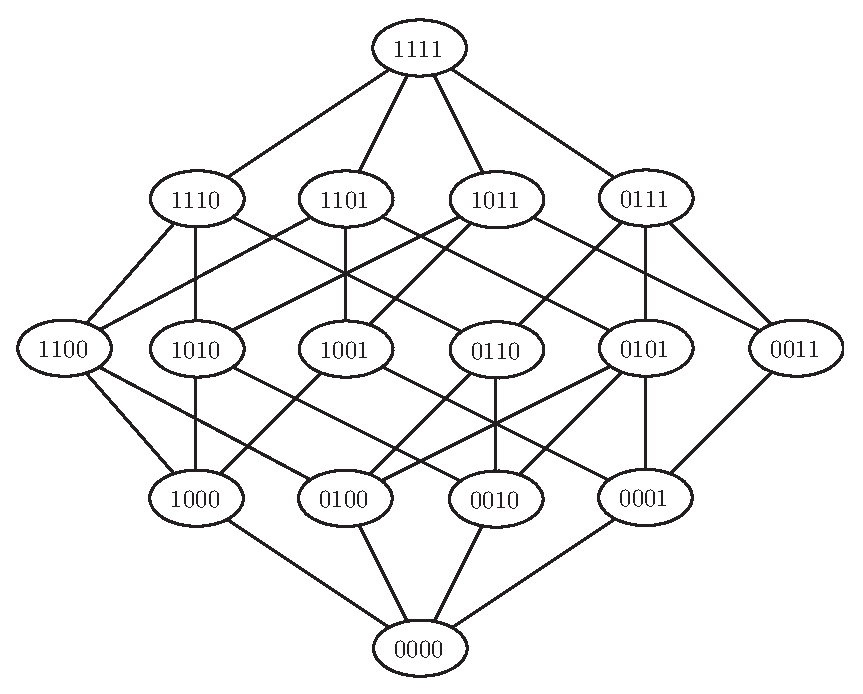
\includegraphics [scale = 0.6]{images/cube-booleen.eps}
    \end{center}
    \caption{Boolean cube $ (\FF_2)^4 $}
              \label{fig-cube-booleen}
\end{figure}
 
% ------------------------------------------------- -----
% ------------------------------------------------- -----
% sub-section - Presentation                            
% ------------------------------------------------- -----
% ------------------------------------------------- -----
\subsection{Presentation}
\label{sect2-presentation-transforme-walsh} 
 
 
By closely following the proof of the corollary \ref{cor-thm-isomorphism}, we can easily construct the dual of a group which is written as a product of elementary cyclic groups. Indeed, each character will be expressed as a product of the different characters of the elementary groups. In the case of the group $ (\ZZ/2 \ZZ)^k $, this is extremely simple, since the only non-trivial character of the group $ \ZZ/2 \ZZ = \{0,1\} $ is defined through
\begin{equation*}
\chi_{\epsilon} (0) = 1 \quad \quad \chi_{\epsilon} (1) = -1.
\end{equation*}
To each element $ a = \{a_0, \ldots, \, a_{k-1}\} \in (\ZZ/2 \ZZ)^k $ we can therefore assign a character
\begin{equation}
\label{eq-denf-base-walsh}
\chi_a: \func{(\ZZ/2 \ZZ)^k}{\{- 1, \, 1\}}{x = \{x_0, \ldots, \, x_{k-1}\}}{(-1)^{a_0 x_0} (-1)^{a_1 x_1} \cdots (-1)^{a_{k-1} x_{k-1}} = (-1)^{\dotp{a}{x}}}.
\end{equation}
where we have denoted $ \dotp{a}{x} $ the canonical bilinear form over $ (\ZZ/2 \ZZ)^k $ defined by
\begin{equation*}
\dotp{a}{x} \eqdef \sum_{i = 0}^{k-1}{a_i x_i}.
\end{equation*}
In practice, we represent the elements of the group $ (\ZZ/2 \ZZ)^k $ as integers between $ 0 $ and $ 2^k-1 $, by assimilating the element $ x \in G = (\ZZ/2 \ZZ)^k $ with the integer $ \sum_{i = 0}^{k-1}{x_i 2^i} $. This allows to see the characters $ \chi_a $ (where $ a $ can be seen as an element of $ G $ or as an integer of $ \{0, \ldots, \, 2^k-1\} $) as vectors of size $ 2^k $ filled with $ -1 $ and $ 1 $.
 
\begin{exmp}
\index{Matrix!of Walsh} \label{notation-32} Consider the group $ (\ZZ/2 \ZZ)^3 $, of cardinal 8. We can represent its character table as a square matrix of order 8 , denoted $ W_8 $, whose line $ i $ represents the values of the character $ \chi_i $, that is to say that $ (W_8)_{ij} = \chi_i (j) $. Here is the table:
\begin{equation}
\label{eqn-matrix-walsh-8}
W_8 \eqdef \begin{pmatrix} 1 & 1 & 1 & 1 & 1 & 1 & 1 & 1 \\1 & -1 & 1 & -1 & 1 & -1 & 1 & -1 \\1 & 1 & -1 & -1 & 1 & 1 & -1 & -1 \\1 & -1 & -1 & 1 & 1 & -1 & -1 & 1 \\1 & 1 & 1 & 1 & -1 & - 1 & -1 & -1 \\1 & -1 & 1 & -1 & -1 & 1 & -1 & 1 \\1 & 1 & -1 & -1 & -1 & -1 & 1 & 1 \\1 & -1 & -1 & 1 & -1 & 1 & 1 & -1 \end{pmatrix}.
\end{equation}
The figure \figref{fig-matrices-walsh} shows the Walsh matrix $ W_{64} $, where we have made the entries equal to $ 1 $ white, and those equal to $ -1 $ in black. \begin{figure}[ht] 
    \begin{center}
    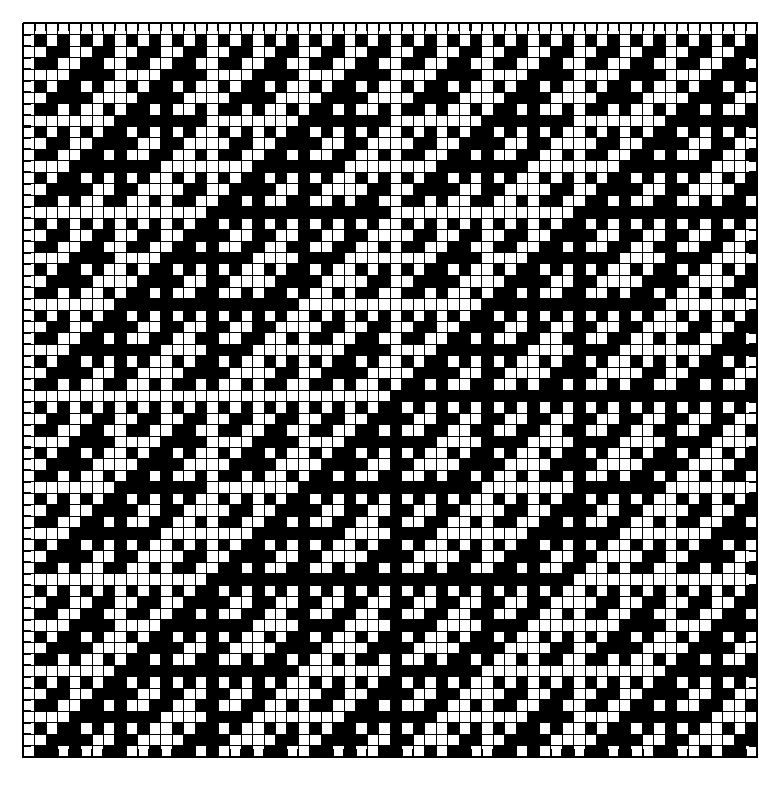
\includegraphics [scale = 0.4]{images/matrices-walsh.eps}
    \end{center}
    \caption{Walsh matrix $ W_{64} $}
              \label{fig-matrices-walsh}
\end{figure}
\end{exmp}
We can then define the \textit{Walsh transform}.
 
\begin{defn}[Walsh transform]
\index{Walsh transform} \label{notation-33} We define the \textit{Walsh transform} $ \Ww_k (f) $ of a complex vector $ f = \{f [0], \ldots, \, f [2^k-1]\} $ of size $ 2^k $ by
\begin{equation}
\label{eq-formula-defn-trans-walsh}
\forall i \in \{0, \ldots, \, 2^k-1\}, \quad \Ww_k (f) [i] \eqdef \sum_{j = 0}^{2^k-1}{f [j] \chi_i (j)} = 2^k \dotp{f}{\chi_i}.
\end{equation}
\end{defn}
 
 
\begin{rem}{(\upshape \textbf{Link with the Fourier transform}).} 
We should also note $ f: (\ZZ/2 \ZZ)^k \rightarrow \CC $ the function corresponding to the vector $ f $, that is to say the vector corresponding to the decomposition of $ f $ in the basis of Dirac functions $ \{\delta_x\}_{x \in G} $. Then the computation of $ \Ww (f) $ is that of a Fourier transform, since
\begin{equation*}
\Ww (f) [i] = 2^k \dotp{f}{\chi_i} = \wh{f} (\chi_i),
\end{equation*}
where we have denoted $ \wh{f}: \wh{G} \rightarrow \CC $ the Fourier transform of $ f $. In particular, we will therefore be able to state without effort the inversion formula for the Walsh transform.
\end{rem}
If we represent the frequencies $ i \in \{0, \ldots, \, 2^n-1\} $ on the boolean cube of the figure \figref{fig-cube-booleen}, then the frequencies located in bottom of the diagram are often referred to as \textit{low frequencies}. We find many analogies with the Fourier spectra already encountered (Fourier transforms on a finite group, continuous transform, etc.). Thus, the exercise \oldref{exo-learning-boolean-functions} proposes to use the spectral properties of the Walsh transform to perform boolean predictions (this is related to the \textit{theory of learning}) .
 
 
The operator $ \Ww_k: \CC^{2^k} \rightarrow \CC^{2^k} $ is a linear map whose matrix in the canonical basis is $ W_{2^k} $, the table of characters in the group $ (\ZZ/2 \ZZ)^k $. We thus have $ \Ww_k (f) = W_{2^k} f $. The inversion formula obtained from the proposition \ref{prop-decomposition-serie-fourier}, gives us the following information.
 
\begin{prop}
\label{prop-pte-matrix-hadamard}
\index{Inversion formula} The Walsh transform is invertible, and its inverse is $ \frac{1}{2^k} \Ww_k $. From a matrix point of view, this means that the matrix $ W_{2^k} = \{w_{ij}\} $, defined by $ w_{ij} = (-1)^{\dotp{i}{j}} $, check $ W_{2^k} W_{2^k} = 2^k Id $.
\end{prop}
The Walsh matrix makes it possible to study concrete problems, for example in statistics, as shown by the exercise \oldref{exo-transforme-walsh-statistic}.

% ------------------------------------------------- -----
% ------------------------------------------------- -----
% sub-section - Fast calculation algorithm                            
% ------------------------------------------------- -----
% ------------------------------------------------- -----
\subsection{Fast calculation algorithm}
\label{sect2-fwt} 
 
 
\index{Divide and conquer} One of the advantages of the Walsh transform is that we have a fast algorithm to calculate it. Indeed, although the equation that defines it may seem a bit complicated, it can be broken down in a simple way. This will make it possible to implement a recursive calculation algorithm, much more efficient than the naive evaluation of the sum which defines the transform. We will study in the next chapter the construction of \textit{the FFT algorithm}, and we will find exactly the same ideas, which are at the base of the algorithmic \guill{philosophy} called \textit{divide and conquer}.
 
 
\index{Algorithm!FWT} Rather than spending time on the analysis of such an algorithm (its cost, its implementation, etc.), we will simply describe the recurrence equation that we will put into{\oe } work. Discussions on the efficiency of such an implementation are postponed to the next chapter, about \textit{the FFT algorithm}. Here is the famous idea which is the basis of our algorithm. We need to rewrite the equation \eqref{eq-formula-defn-trans-walsh}, as follows:
\begin{equation*}
\Ww_k (f) [i] = \sum_{j = 0}^{2^{k-1} -1}{f [j] (-1)^{\sum_{p = 0}^{k- 2}{j_p i_p}}} + (-1)^{i_{k-1}} \sum_{j = 0}^{2^{k-1} -1}{f [j + 2^{k -1}] (-1)^{\sum_{p = 0}^{k-2}{j_p i_p}}}.
\end{equation*}
To write this expression in a simpler way, we introduce the vectors $ f_1 $ and $ f_2 $ of length $ 2^{k-1} $ defined as follows:
\begin{equation*}
\forall j \in \{0, \ldots, \, 2^{k-1} -1\}, \quad f_1 [j] = f [j] \quad \text{and} \quad f_2 [j] = f [j + 2^{k-1}].
\end{equation*}
Similarly, we will write $ \Ww_k (f)_1 $ (respectively $ \Ww_k (f)_2 $) to denote the $ 2^{k-1} $ prime (respectively last) indices of the transformed vector $ \Ww_k (f) $. We then have the recurrence equation
\begin{equation*}
\begin{split}
\Ww_k (f)_1 & = \Ww_{k-1} (f_1) + \Ww_{k-1} (f_2) \\
\Ww_k (f)_2 & = \Ww_{k-1} (f_1) - \Ww_{k-1} (f_2).
\end{split}
\end{equation*}
From a matrix point of view this decomposition is written in the form
\begin{equation*}
W_{2^k} = \begin{pmatrix} W_{2^{k-1}} & W_{2^{k-1}} \\W_{2^{k-1}} & -W_{2^{k-1}} \end{pmatrix}.
\end{equation*}
\index{Tensor product} The decomposition of $ W_{2^k} $ found corresponds to a tensor product structure, as specified in the exercise \oldref{exo-tensor-product}. \index{Matlab@\Matlab{}} This decomposition quite naturally gives rise to a very fast calculation algorithm, named \textit{FWT} for \textbf{F} ast \textbf{W} alsh \textbf{T} ransform. More precisely, if we count the number of additions necessary to calculate the Walsh transform of a vector of size $ n = 2^k $, we see that we obtain $ k = \log_2 (n ) $ recursive calls, with each time $ n $ additions or subtractions. Hence a cost of $ n \log_2 (n) $ operations. This is a substantial gain over the naive implementation of the \eqref{eq-formula-defn-trans-walsh} equation, which requires $ n^2 $ operations. The \listingterme{} \Matlab{} of this algorithm is presented in paragraph \annexeref{sect1-listing-fwt}.

% ------------------------------------------------- -----
% ------------------------------------------------- -----
% sub-section - Using the Walsh transform                            
% ------------------------------------------------- -----
% ------------------------------------------------- -----
\subsection{Use of the Walsh transform}
\label{sect2-use-fwt} 
 
 
\index{Base!orthogonal} The main interest of the Walsh transform is that it allows to decompose any function from $ \{0, \ldots, \, 2^k-1\} $ into $ \CC $ on the orthogonal basis of the characters of $ (\FF_2)^k $. More precisely, we have
\begin{equation*}
\forall i \in \{0, \ldots, \, 2^k-1\}, \quad f [i] = \frac{1}{2^k} \sum_{j = 0}^{2^{k-1}}{\Ww_k (f) [j] \chi_j (i)}.
\end{equation*}
This transform is very quick to use, because it only uses addition and subtraction (no multiplication). In addition, we have seen that we have a formidably efficient algorithm for recursively calculating the Walsh transform . However, the Walsh transform has a weak point of size: it has no pleasant property with respect to the convolution of the functions of $ \{0, \ldots, \, 2^k-1\} $ in $ \CC $, unlike the Fourier transform, as we saw in paragraph~\ref{sect2-convolution-transforme-fourier}. Indeed, the Walsh transform is a Fourier transform on the binary cube $ (\ZZ/2 \ZZ)^k $, not at all on the cyclic group $ \ZZ/2^k \ZZ $. It is mainly because of this that we will be led in the next chapter to study more closely the Fourier transform on a cyclic group. This will allow us to build an algorithm to compute convolutions on $ \ZZ/2^k \ZZ $ extremely fast.
 
 
\index{Compression} The exercise \oldref{exo-compression-walsh} shows how we can use the Walsh transform to achieve \textit{signal compression}. He also proposes to extend the Walsh transform to the two-dimensional frame.
 
 
\index{Function!boolean} \index{Non-linearity} Finally, the Walsh transform allows us to study \textit{boolean functions}, and in particular their \textit{non-linearity}. As this study supposes to consider functions with values in the finite-field $ \FF_2 $, it is approached only at the end of the chapter \oldref{chap-extension-finite-field-values}, at exercise \oldref{exo-boolean-functions}. In the same vein, the exercise \oldref{exo-learning-boolean-functions} introduces probabilistic notions to study Boolean functions and their learning.
% ------------------------------------------------- -----
% ------------------------------------------------- -----
% ------------------------------------------------- -----
% section - Poisson formula                            
% ------------------------------------------------- -----
% ------------------------------------------------- -----
% ------------------------------------------------- -----
\section{Poisson formula}
% \addcontentsline{toc}{section}{Poisson formula}
\label{sect1-fish-formula} 
 
\index{Identity!of MacWilliams} \index{MacWilliams@\nompropreindex{MacWilliams}} We have seen, in particular in Paragraph~\ref{sect2-bidual} devoted to bidual, the great similarity between duality on a finite abelian group, and duality on a vector space. In this paragraph, we will give another embodiment of this fact, in this case by studying the notion of orthogonality between a group and its dual. The central point of this approach is the \textit{Poisson formula}. We will thus see that if we apply this formula in the case of a group which is also a vector space (on a finite field), we obtain very powerful relations, called identities of \textit{MacWilliams}.
% ------------------------------------------------- -----
% ------------------------------------------------- -----
% sub-section - The formula on a finite abelian group                            
% ------------------------------------------------- -----
% ------------------------------------------------- -----
\subsection{The formula on a finite abelian group}
\label{abelian-finite-grpe-fish-formula} 
 
 
Before stating the Poisson formula on a finite group, it is necessary to clarify the notion of orthogonality. Let us start by briefly recalling the theory of orthogonality on a vector space. For a fuller description, we can refer to the work of \nompropre{Ramis}, \nompropre{Dechamps} and \nompropre{Odoux} \cite{ramis-1}.
 
 
\index{Orthogonal!of a vector space} \index{Dual!of a vector space} \label{notation-34} \label{notation-35} \label{notation-36} \index{Duality hook } If $ E $ is a finite dimensional $k$-vector space, we denote by $ E^* \eqdef \Hom (E, \, k) $ its dual, which is made up of linear forms. We classically define a bilinear form on $ E^* \times E $, which we call the hook of duality, as follows:
\begin{equation*}
\forall (f, \, x) \in E^* \times E, \quad \dotp{x}{f} \eqdef f(x).
\end{equation*}
We then define, for a part $ A \subset E $, its orthogonal
\begin{equation}
\label{eq-defn-orthogonal-ev}
A^{\bot} \eqdef \enscond{f \in E^*}{\forall x \in A, \; \dotp{x}{f} = 0}.
\end{equation}
We verify that it is a vector subspace of $ E $, and we have $ E^{\bot} = \{0\} $. Similarly, we define the orthogonal of $ B \subset E^* $ by
\begin{equation*}
B^{0} = \enscond{x \in E}{\forall f \in B, \; \dotp{x}{f} = 0}.
\end{equation*}
It is a vector subspace of $ E^* $, and we have $ (E^*)^0 = \{0\} $. Note that these properties are still true in infinite dimension, but we must use the axiom of choice. In \textit{finite} dimension, the maps $ F \mapsto F^{\bot} $ and $ G \mapsto G^0 $ are reciprocal bijections between subspaces of $ E $ and $ E^* $. They reverse inclusion.
 
 
Once in memory these linear notions of orthogonality, it is natural to introduce the following definition:
 
\begin{defn}[Orthogonal of a subgroup]
\label{defn-orthogonal-abelian-subgroup}
\index{Orthogonal!of a subgroup} \index{Subgroup} \label{notation-37} Let $ G $ be a finite abelian group, and $ H \subset G $ a subgroup. We denote by $ H^{\sharp} $ the orthogonal of $ H $ which is the subgroup of $ \wh{G} $ defined as follows:
\begin{equation*}
H^{\sharp} \eqdef \enscond{\chi \in \wh{G}}{\forall h \in H, \; \chi (h) = 1}.
\end{equation*}
\end{defn}

We have already seen during the demonstration of the lemma \ref{lem-suite-exact}, that any trivial character of $ \wh{G} $ over $ H $ is uniquely identified with an element of $ \wh{G / H} $, and vice versa. More precisely, we have an isomorphism $ H^{\sharp} \simeq \wh{G / H} $. We therefore see that $ H^{\sharp} $ is a subgroup of $ \wh{G} $ of cardinality $ |G| / | H | $. For example, we have $ G^{\sharp} = \{1\} $. In addition, the application $ H \mapsto H^{\sharp} $ reverses inclusions. Here again, the resemblance to the duality between the vector spaces is striking.
 
 
We can now state the \textit{Poisson formula} in the framework of finite abelian groups.
 
\begin{thm}[Poisson formula]
\index{Poisson's formula} \index{Poisson@\nompropreindex{Poisson}} Let $ G $ be a finite abelian group, and $ H \subset G $ a subgroup. So, for $ f: G \rightarrow \CC $, that is to say $ f \in \CC [G] $, we have
\begin{equation}
\label{eq-formula-fish-finished-grp}
\forall g \in G, \quad \sum_{h \in H}{f(gh)} = \frac{| H |}{|G|} \sum_{\chi \in H^{\sharp}}{\wh{f} (\ol{\chi}) \chi (g)}.
\end{equation}
We denote by $ \wh{f}: \wh{G} \rightarrow \CC $ the Fourier transform of $ f $.
\end{thm}

\begin{proof}
\index{Translation} To simplify the notations, we consider $ S $ a system of representatives of $ G / H $ in $ G $. We denote by $ \ol{g} $ the image of $ g \in S $ in $ G / H $ (that is to say the image by canonical projection). Let's start by defining a function $ \wt{f} $ on $ G / H $ by
\begin{equation*}
\forall g \in S, \quad \wt{f} (\ol{g}) \eqdef \sum_{h \in H}{f(gh)}.
\end{equation*}
This amounts to replacing $ f $ by an invariant function under the translation by elements of $ H $ (we \guill{periodize}). We see that this function is defined without ambiguity, since, if we consider another representative $ g'$ of the class $ g H $, we have $ g' = g h'$ with $ h' $ an element of $ H $, and therefore, $ \wt{f} (\ol{g}) = \wt{f} (\ol{g'}) $. We can therefore decompose the function $ \wt{f} \in \CC [G / H] $ into a Fourier series:
\begin{equation}
\label{eq-demo-formuel-fish-gpe-finite-tmp}
\forall g \in S, \quad \wt{f} (\ol{g}) = \sum_{\chi \in \wh{G / H}}{\dotp{\wt{f}}{\chi } \chi (\ol{g})}.
\end{equation}
We can then explain the value of the Fourier coefficients:
\begin{equation}
\label{eq-formula-fish-intermediate-result}
\dotp{\wt{f}}{\chi} = \frac{1}{| G / H |} \sum_{g \in S}{\wt{f} (\ol{g}) \ol{\chi (\ol{g})}} = \frac{| H |}{|G|} \sum_{g \in S}{\sum_{h \in H}{f(gh) \ol{\chi (\ol{g})}}}.
\end{equation}
Noticing that the application
\begin{equation*}
\func{S \times H}{G}{(g, \, h)}{gh}
\end{equation*}
is a bijection and using the fact that for $ \chi \in \wh{G / H} $, $ \chi (\ol{gh}) = \chi (\ol{g}) $, we can rewrite the sum \eqref{eq-formula-fish-intermediate-result} in the form
\begin{equation*}
\dotp{\wt{f}}{\chi} = \frac{| H |}{|G|} \sum_{g \in G}{f(g) \ol{\chi (g)}} \eqdef \frac{| H |}{|G|} \wh{f} (\ol{\chi}).
\end{equation*}
All that remains is to report the value of these coefficients in the equation \eqref{eq-demo-formuel-fish-gpe-finite-tmp} and notice that the expression of $ \wt{f} (\ol{g}) $ gives us the left side of the Poisson formula.
\end{proof}
By applying the equation \eqref{eq-formula-fish-finished-grp} with $ g = 1 $, we obtain the form in which the formula is often written:
\begin{equation}
\label{eq-formula-fish-group-finite-simple}
\sum_{h \in H}{f(h)} = \frac{| H |}{|G|} \sum_{\chi \in H^{\sharp}}{\wh{f} (\chi )}.
\end{equation}
In order to better understand the Poisson formula, we will give another proof, which uses only linear algebra arguments on the vector space $ \CC [G] $. Before giving this proof, let us study more precisely the space $ \CC [G / H] $.
 
If we denote by $ \pi: G \rightarrow G / H $ the canonical projection, we can define an application
\begin{equation*}
\pi^*: \func{\CC [G / H]}{\CC [G]}{f}{f \circ \pi}.
\end{equation*}
$ \pi^* $ is in fact an injective linear map (because $ \pi $ is surjective). The space $ \CC [G / H] $ is therefore identified with a vector subspace of $ \CC [G] $, which is in fact formed by constant functions on each of the classes on the left modulo $ H $. To demonstrate this fact, it suffices to note that $ \pi^* $ can be inverted on its image as follows:
\begin{equation*}
(\pi^*)^{-1} \func{\Im (\pi^*)}{\CC [G / H]}{f}{\wt{f}},
\end{equation*}
where we denote by $ \wt{f} (\ol{x}) $ (for $ x \in G $) the value of $ f $ on the class to the left of $ x $ modulo $ H $. This identification being made, we can give a new proof of the Poisson formula.
 
 
\begin{proof}
As before, we fix a function $ f \in \CC [G] $. Recall that the space $ \CC [G] $ is endowed with an algebra structure thanks to the convolution product $ * $, whose expression is given to the equation \eqref{eq-formula-prod-convol-grpe-abelien}. We can then consider a filtering operator
\begin{equation*}
\Phi^f: \func{\CC [G]}{\CC [G]}{\varphi}{f * \varphi}.
\end{equation*}
We will see in the Section~\ref{sect1-filtering}, why we call such operators filter operators. By using the identification between the functions of $ \CC [G / H] $ and the functions of $ \CC [G] $ constants on the classes on the left $ g H $, we can show that $ \CC [G / H] $ is a subspace of $ \CC [G] $ stable by $ \Phi^f $. Indeed, if we give ourselves $ \varphi $ constant on the classes on the left, and $ g'= g h' $, for $ g \in G $ and $ h'\in G $, we obtain
\begin{equation*}
\Phi^f(\varphi) (g') = \sum_{x \in G}{f(gh' x^{-1}) \varphi (x)} = \sum_{x \in G}{f(g (xh'^{-1})^{-1}) \varphi (x h'^{-1})} = \Phi^f(\varphi) (g).
\end{equation*}
This being shown, we can therefore consider $ \wt{\Phi}^f $, the restriction of $ \Phi^f $ to $ \CC [G / H] $. The trick to finding the Poisson formula is to calculate the trace of $ \wt{\Phi}^f $. We have an obvious basis of $ \CC [G / H] $, namely $ \Bb \eqdef \{\delta_g\}_{g \in S} $ (we always denote $ S $ a system of representative of $ G / H $). We recall that $ \delta_g $ is the function which is worth $ 1 $ in $ g $, and $ 0 $ everywhere else. In this base, the expression of the operator trace is simple to calculate, since the calculation of the images of the base vectors gives
\begin{equation*}
\forall s \in S, \quad \wt{\Phi}^f(\delta_s): g \mapsto \sum_{x \in S}{\sum_{h \in H}{f(gx^{- 1 } h^{-1}) \delta_s (x)}},
\end{equation*}
because we must remember that $ \delta_s $ is seen as a constant function on the classes on the left. As a result, we get
\begin{equation*}
\forall s \in S, \quad \wt{\Phi}^f(\delta_s): g \mapsto \sum_{h \in H}{f(gs^{-1} h^{-1})} .
\end{equation*}
The trace is therefore calculated effortlessly:
\begin{equation*}
\Tr \left(\wt{\Phi}^f \right) = \sum_{s \in S}{\sum_{h \in H}{f(ss^{-1} h^{-1}) }} = \frac{|G|}{| H |} \sum_{h \in H}{f(h)}.
\end{equation*}
Up to a constant, we get the left side of the Poisson formula. To obtain the right-hand side, it will suffice to calculate the trace of $ \wt{\Phi}^f $ in another base. And of course, we are going to reinvest the work done in the previous chapter by choosing the orthonormal basis of the characters of $ G / H $, that is to say the elements of $ H^{\sharp} $. The advantage is that the characters behave in a particularly pleasant way vis-à-vis the convolution. Indeed, the convolution theorem \ref{thm-convolution-trans-fourier-grpe-abelien}, allows to show that the elements of $ H^\sharp $ are the eigenvectors of the operator $ \wt{\Phi }^f $, since
\begin{equation*}
\forall \chi \in \wh{G / H} = H^{\sharp}, \quad \wt{\Phi}^f(\chi) = \wh{f} (\chi) \chi.
\end{equation*}
The exercise \oldref{exo-determinant-circulating}, question 1, details the proof of this. It only remains to exploit the fact that the trace of the operator $ \wt{\Phi}^f $ is equal to the sum of its eigenvalues, to conclude that
\begin{equation*}
\Tr \left(\wt{\Phi}^f \right) = \sum_{\chi \in H^{\sharp}}{\wh{f} (\chi)}.
\end{equation*}
We therefore find the simplified Poisson formula \eqref{eq-formula-fish-group-finite-simple}. To obtain the complete equation \eqref{eq-formula-fish-finished-grp}, it suffices to apply the obtained equation to the function $ f_g: x \rightarrow f(gx) $, for $ g \in G $, since we have
\begin{equation*}
\forall \chi \in \wh{G}, \quad \wh{f_g} (\chi) = \chi (g^{-1}) \wh{f} (\chi).
\end{equation*}
This reasoning shows moreover that the equations \eqref{eq-formula-fish-group-finite-simple} and \eqref{eq-formula-fish-finished-grp} are completely equivalent.
\end{proof}
 
% ------------------------------------------------- -----
% ------------------------------------------------- -----
% sub-section - Application to MacWilliams identities                            
% ------------------------------------------------- -----
% ------------------------------------------------- -----
\subsection{Application to MacWilliams identities}
\label{sect2-application-id-mac-williams} 
 
 
In this paragraph, we will use the Poisson formula as part of the group $ G $ equal to $ (\ZZ/2 \ZZ)^k = (\FF_2)^k $. We are therefore going to place ourselves in the framework where we carried out the study of the Walsh transform (Section~\ref{sect1-transforme-walsh}), and we will use the same notations. The interest of such a group is that it is in addition a vector space, in this case on the finite field $ \FF_2 $. In reality, the situation is very simple, since the notion of subgroup coincides with that of vector subspace (the group operation corresponds to the addition of vectors, and since the field has only two elements, the multiplication of a vector by a scalar is an operation which trivially respects the subgroup structure). We therefore do not lose information by translating the statements resulting from duality over a group (Poisson's formula) into the language of linear algebra. We will see that in this framework, the notions of duality and orthogonality are the same for the two structures.
 
 
All the study made in this paragraph generalizes without modification to the case of the vector space $ K^k $, where $ K $ is any finite field. The exercise \oldref{exo-generalization-mac-williams} takes this construction step by step. However, to stay within the framework developed for the Walsh transform, we will restrict ourselves to the case of the space $ (\FF_2)^k $.
 
 
Remember that we have a complete description of the dual $ \wh{F_2^k} $, since at each element $ a = \{a_0, \ldots, \, a_{k-1}\} \in ( \ZZ/2 \ZZ)^k $ we match a character
\begin{equation*}
\chi_a: \func{(\ZZ/2 \ZZ)^k}{\{- 1, \, 1\}}{x = \{x_0, \ldots, \, x_{k-1}\}}{(-1)^{\dotp{a}{x}}}.
\end{equation*}
This allows us to calculate, for a group $ H \subset G $, the orthogonal $ H^{\sharp} $. Indeed, to say that $ \chi_a \in H^{\sharp} $ is equivalent to
\begin{equation*}
\forall h \in H, \quad \chi_a (h) = (-1)^{\dotp{a}{h}} = 1.
\end{equation*}
This therefore means that
\begin{equation}
\label{eq-equivalence-orthogonalite-caractere}
\forall h \in H, \quad \dotp{a}{h} = 0 \Leftrightarrow a \in H^{\bot},
\end{equation}
where we have denoted $ H^{\bot} $ the orthogonal of $ H $ when we consider $ H $ as a vector subspace of $ (\FF_2)^k $. This orthogonal can of course be seen as the orthogonal for the canonical symmetric bilinear form on $ (\FF_2)^k $. We can also see it as the orthogonal in the sense of duality (definition \eqref{eq-defn-orthogonal-ev}), if we have identified the vector space $ (\FF_2)^k $ and its dual by identifying the canonical base with its dual base. However, be careful that the orthogonal space $ H^\bot $ has no reason to be an additional of $ H $, for example, in $ (\FF_2)^4 $, the vector $ ( 1, \, 1, \, 1, \, 1) $ is orthogonal to itself. The exercise \oldref{exo-codes-autoduaux} precisely studies the cases where the space $ H $ coincides with its dual (it uses the language of error correcting codes and group actions).
 
 
In the end, if we identify the elements $ a \in G $ and $ \chi_a \in \wh{G} $, we obtain the remarkable property that $ H^{\sharp} = H^{\bot} $ . We can now state the Poisson formula in terms of vector spaces.
 
\begin{prop}[Vector Poisson formula]
\label{prop-formula-vector-fish}
\index{Vector Poisson's Formula} Let $ H $ be a vector subspace of $ (\FF_2)^k $. Let $ f $ be a function $ f: (\FF_2)^k \rightarrow \CC $. We then have the two relations
\begin{align}
\label{eq-formula-fish-vector-1}
\sum_{a \in H}{f(a)} & = \frac{| H |}{2^k} \sum_{u \in H^{\sharp}}{\wh{f} (\chi_u )}. \\
\label{eq-formula-vector-fish-2}
\sum_{a \in H^{\sharp}}{f(a)} & = \frac{1}{| H |} \sum_{u \in H}{\wh{f} (\chi_u)} .
\end{align}
Remember that
\begin{equation*}
\wh{f} (\chi_u) \eqdef \sum_{x \in (\FF_2)^k}{(-1)^{\dotp{u}{x}} f(x)}.
\end{equation*}
\end{prop}
\begin{proof}
The first equation is the exact translation of the Poisson formula, with the identification $ H^{\bot} = H^{\sharp} $ that we have updated. For the second equation, it suffices to replace in the first $ H $ by its orthogonal $ H^{\bot} $. Like $ | H^{\bot} | = \frac{| (\FF_2)^k |}{| H |} $, we get the desired result.
\end{proof}
 
 
 
We will now be able to apply the Poisson formula for combinatorial purposes. The goal of this study is to better understand the structure of the space $ (\FF_2)^k $ when it is provided with a somewhat particular distance, which we call the distance of \textit{Hamming}. For now, it is above all a computational exercise, which will reveal some rather spectacular relationships. However, we will see in Section~\ref{sect1-applications-correctors-codes}, that all of this has applications in the study of binary corrective codes. But let us content ourselves, first of all, with defining this famous distance.
 
\begin{defn}[Hamming distance]
\index{Distance!from Hamming} \label{notation-38} \label{notation-39} Let $ x $ and $ y \in (\FF_2)^k $. We define the \textit{Hamming distance} $ d (x, \, y) $ between these two vectors as follows:
\begin{equation*}
d (x, \, y) \eqdef w (xy) \quad \text{with} \quad w (z) = \sharp \enscond{i = 0, \ldots, \, k-1}{z_i \neq 0}.
\end{equation*}
We call $ w (z) $ the weight of the vector $ z $.
\end{defn}
 
 
 
The figure \figref{fig-cube-booleen} represents the group $ (\FF_2)^4 $ where we have connected the elements at a distance of 1. In order to study the structure of a subspace $ H $ with respect to the distance $ d $, we are interested in the weight distribution of the words that form $ H $. The following definitions are then introduced.
 
\begin{defn}[Enumerator polynomial]
\index{Polynomial!enumerator} \label{notation-40} Let $ H $ be a vector subspace of $ (\FF_2)^k $. We denote by $ A_H \in \ZZ [X, \, Y] $ the \textit{enumerator polynomial of weight} of $ H $, which is defined by
\begin{equation*}
A_H (X, \, Y) \eqdef \sum_{c \in H}{X^{kw (c)} Y^{w (c)}} = \sum_{i = 0}^{k}{A_i X^{ki} Y^i},
\end{equation*}
where we denote by $ A_i $ the number of vectors of $ H $ of weight $ i $.
\end{defn}
The following relation, discovered by \nompropre{MacWilliams}, relates the weights of the words in the space $ H $ with the weights of the words of its orthogonal.
 
\begin{thm}[MacWilliams identity]
\label{thm-id-mac-williams}
\index{Identity!of MacWilliams} \index{MacWilliams@\nompropreindex{MacWilliams}} Let $ H $ be a vector subspace of $ (\FF_2)^k $. We then have
\begin{equation*}
A_{H^{\bot}} (X, \, Y) = \frac{1}{| H |} A_{H} (X + Y, \, XY).
\end{equation*}
\end{thm}
\begin{proof}
Let $ x $ and $ y $ be two fixed complex numbers. We then define the function $ f \in \CC [(\FF_2)^k] $ by
\begin{equation*}
\forall a \in (\FF_2)^k, \quad f(a) \eqdef x^{kw (a)} y^{w (a)}.
\end{equation*}
In order to apply the Poisson formula, we need to calculate $ \wh{f} $:
\begin{equation*}
\forall a \in (\FF_2)^k, \quad \wh{f} (\chi_a) \eqdef \sum_{t \in (\FF_2)^k}{x^{kw (t)} y^{w (t)} (-1)^{\dotp{t}{a}}}.
\end{equation*}
Using the fact that $ w (t) = \sum_{i = 0}^{k-1}{t_i} $ in $ \NN $, where $ t_i \in \{0, \, 1\} $, we obtain
\begin{equation*}
\forall a \in (\FF_2)^k, \quad \wh{f} (\chi_a) = \sum_{t \in (\FF_2)^k}{\prod_{i = 0}^{k-1 }{x^{1-t_i} y^{t_i} (- 1)^{a_i t_i}}} = \prod_{i = 0}^{k-1}{\sum_{t_i = 0}^1{x^{k-t_i} y^{t_i} (-1)^{a_i t_i}}}.
\end{equation*}
If $ a_i = 0 $, the inner sum is worth $ x + y $, while if $ a_i = 1 $, we find $ xy $. So we have
\begin{equation*}
\forall a \in (\FF_2)^k, \quad \wh{f} (\chi_a) = (x + y)^{kw (a)} (xy)^{w (a)}.
\end{equation*}
We can now apply the Poisson formula \eqref{eq-formula-vector-fish-2}. The equality of the theorem is thus true if we consider the values of the polynomials whatever the point $ (x, \, y) \in \CC^2 $. It is therefore also true as a polynomial equality over $ \ZZ [X, \, Y] $.
\end{proof}
 
 
 
This identity, in addition to its certain aesthetic interest, constitutes the main tool for the combinatorial study of corrective codes. The Section~\ref{sect1-codes-correctors-duality}, reformulates the identity of MacWilliams within the framework of code theory, and explains the multiple applications which result from it.

% ------------------------------------------------- -----
% ------------------------------------------------- -----
% sub-section - The Poisson formula continues                            
% ------------------------------------------------- -----
% ------------------------------------------------- -----
\subsection{The continuous Poisson formula}
 
 
\index{Poisson's formula!continuous} The Poisson formula we just used on a finite abelian group actually has a similar statement in the context of continuous functions defined on $ \RR $. To make this statement pleasant, we will define the continuous Fourier transform as follows:
\begin{equation}
\label{eq-defn-trans-fourier-special-fish}
\forall f \in L^1 (\RR), \forall x \in \RR, \quad \wh{f} (x) \eqdef \int_{\RR}{f(t) e^{- 2 \imath \pi tx} \d t}.
\end{equation}
We can then state the Poisson formula on $ \RR $. It will be noted with great interest that its proof is largely similar to that made in the framework of finite groups. The only difficulty of the continuous case lies in the problems of convergence of the manipulated series, which obliges us to impose more restrictive assumptions on the functions that we analyze.
 
\begin{thm}[Continuous Poisson formula]
\label{thm-formula-fish-continue}
Let $ f \in L^1 (\RR) $ be a continuous function such that
\begin{align}
\label{eq-formula-fish-hyp1}
& \exists M> 0, \; \exists \alpha> 1, \quad | f(x) | \leq M (1+ | x |)^{- \alpha}, \\
\label{eq-formula-fish-hyp2}
& \sum_{n = \minf}^{\pinf}{| \wh{f} (n) |} <+ \infty.
\end{align}
Under these assumptions, we have
\begin{equation}
\label{eq-formula-fish-continue}
\sum_{n = \minf}^{\pinf}{f(n)} = \sum_{n = \minf}^{\pinf}{\wh{f} (n)}.
\end{equation}
\end{thm}
\begin{proof}
\index{Series!of Fourier} \index{Periodization} We start by periodizing the function $ f $ by introducing the function
\begin{equation*}
\forall x \in \RR, \quad f_1 (x) \eqdef \sum_{n = \minf}^{\pinf}{f(x + n)}
\end{equation*}
If we restrict ourselves to the compact $ \{x \in \RR, \; | x | \leq A\} $, for $ A> 0 $, the hypothesis \eqref{eq-formula-fish-hyp1} allows to affirm, for $ | n | \geq 2A $,
\begin{equation*}
| f(x + n) | \leq M (1+ | x + n |)^{- \alpha} \leq M (1+ | n | -A)^{- \alpha} \leq M (1+ | n | / 2)^{-\alpha},
\end{equation*}
which defines the general term of a convergent series. We therefore conclude that on any compact, the series which defines $ f_1 $ is normally convergent, so that $ f_1 $ is continuous. Moreover, we can easily see that $ f_1 $ is 1-periodic, since
\begin{equation*}
f_1 (x + 1) = \sum_{n = \minf}^{\pinf}{f(x + n + 1)} = \sum_{n'= \minf}^{\pinf}{f(x + n')} = f_1 (x),
\end{equation*}
where we have made the change of variable $ n'= n + 1 $ (authorized by the absolute convergence of the series). We can therefore calculate its Fourier coefficients:
\begin{equation*}
\forall m \in \ZZ, \quad c_m (f_1) = \int_0^1{f_1 (t) e^{- 2 \imath m \pi t} \d t} = \sum_{n \in \ZZ}{\int_0^1{f(t + n) e^{- 2 \imath m \pi t} \d t}},
\end{equation*}
where the inversion between the sum and the integral is justified by the normal convergence of the series of general term $ f(t + n) e^{- 2 \imath m \pi t} $ for $ t \in [0 , 1] $. We can thus continue the calculations to obtain, by changing the variable $ u = t + n $,
\begin{equation*}
\forall m \in \ZZ, \quad c_m (f_1) = \sum_{n \in \ZZ}{\int_{n}^{n + 1}{f(u) e^{- 2 \imath m \pi u}} \d u} = \int_{\minf}^{\pinf}{f(u) e^{- 2 \imath m \pi u} \d u} = \wh{f} (m)
\end{equation*}
(the last equality is justified by Lebesgue's dominated convergence theorem, because $ x \mapsto f(x) e^{- 2 \imath m \pi x} \in L^1 (\RR) $). We therefore note, with the hypothesis \eqref{eq-formula-fish-hyp2} that the Fourier series associated with $ f_1 $ absolutely converges. By additionally using the fact that $ f_1 $ is a continuous function, we therefore conclude that it is the sum of its Fourier series. We can therefore write
\begin{equation*}
\forall x \in \RR, \quad f_1 (x) = \sum_{m \in \ZZ}{c_m (f_1) e^{2 \imath m \pi x}} = \sum_{m \in \ZZ }{\wh{f} (m) e^{2 \imath m \pi x}}.
\end{equation*}
In the end, we therefore obtain equality
\begin{equation*}
\forall x \in \RR, \quad \sum_{n \in \ZZ}{f(x + n)} = \sum_{m \in \ZZ}{\wh{f} (m) e^{2 \imath m \pi x}},
\end{equation*}
which gives the desired Poisson formula by making $ x = $ 0.
\end{proof}
 
 
\begin{rem}{(\upshape \textbf{Link with Poisson's formula on a finite group}).} 
\index{Quotient} \index{Group!quotient} The continuous Poisson formula that we have just demonstrated is in all points similar to the formula \eqref{eq-formula-fish-finished-grp}, valid on a finite abelian group . Indeed, in the continuous case, we must consider the group $ G = \RR^1 $, which is the real line provided with the addition, as well as the discrete subgroup $ \ZZ \subset \RR $. The quotient group is nothing other than the circle $ \RR / \ZZ \simeq S^1 $. Moreover, we will see in Paragraph~\ref{sect2-transforme-fourier-continue}, that we have a complete description of the characters of the circle, since they correspond to the exponentials $ e_n: t \mapsto e^{2 \imath n \pi t} $. We therefore have an explicit isomorphism $ \wh{S^1} \simeq \ZZ $. Therefore, we can write the Poisson formula in the continuous case in the form
\begin{equation*}
\sum_{n \in \ZZ}{f(n)} = \sum_{e_n \in \wh{\RR / \ZZ}}{\dotp{f}{e_n}}.
\end{equation*}
So up to the factor $ \frac{| H |}{|G|} $, this formula is in every way similar to \eqref{eq-formula-fish-finished-grp}.
\end{rem}
 
 
 
\index{Function!Theta of Jacobi} One of the many applications of Poisson's formula concerns the function \textit{Theta} of \textit{Jacobi}, which is defined as follows.
 
\begin{defn}[Jacobi Theta Function]
We define the function \textit{Theta} by
\begin{equation*}
\forall t> 0, \quad \theta (t) \eqdef \sum_{n = \minf}^{\pinf}{e^{- \pi n^2 t}}.
\end{equation*}
\end{defn}
Before stating the functional equation that $ \theta $ satisfies, we need to prove a classical lemma on the Fourier transform of a Gaussian.
 
\begin{lem}
\label{lem-tf-gaussienne}
\index{Gaussian} Let $ g_t $, for $ t> 0 $, be the Gaussian defined by
\begin{equation*}
\forall x \in \RR, \quad g_t (x) = e^{- \frac{x^2}{2t}}.
\end{equation*}
So we have
\begin{equation*}
\forall x \in \RR, \quad \wh{g_t} (x) = \sqrt{2 \pi t} e^{- 2 \pi^2t x^2}
\end{equation*}
where we have kept the definition of the Fourier transform \eqref{eq-defn-trans-fourier-special-fish}.
\end{lem}
\begin{proof}
The transform of the function $ g_t $ is written
\begin{equation*}
\wh{g_t} (x) = \int_{\RR}{e^{- \frac{u^2}{2t}} e^{- 2 \imath \pi ux} \d u}.
\end{equation*}
Using the derivation theorem under the sum sign, we see that the function obtained is $ C^1 $, and that we have
\begin{equation*}
\frac{\d \wh{g_t}}{\d x} (x) = -2 \imath \pi \int_{\RR}{ue^{- \frac{u^2}{2t}} e^{-2 \imath \pi ux} \d u} = -4 \pi^2 xt \wh{g_t} (x),
\end{equation*}
where the last equality is obtained by integration by parts. By solving the differential equation of which $ g_t $ is the solution, we obtain
\begin{equation*}
\wh{g_t} (x) = \wh{g_t} (0) e^{- 2 \pi^2 tx^2}.
\end{equation*}
It only remains to calculate the value of $ \wh{g_t} (0) = \sqrt{t} I $, with $ I = \int_{\RR}{e^{- x^2/2} \d x} $. To do this, it is advisable to switch to polar coordinates when calculating $ I^2 $:
\begin{equation*}
I^2 = \int_{\RR}{\int_{\RR}{e^{- \frac{x^2 + y^2}{2}} \d x} \d y} = 2 \pi \int_0^{\pinf}{re^{- \frac{r^2}{2}} \d r} = 2 \pi.
\end{equation*}
By putting all these results end to end, we get the announced Fourier transform.
\end{proof}
Here is finally the identity of Jacobi on the function $ \theta $.
 
\begin{thm}[Identity of Jacobi]
\index{Identity!of Jacobi}
\begin{equation}
\label{eq-id-jacobi}
\forall t> 0, \quad \theta (t) = \frac{1}{\sqrt{t}} \theta \left(\frac{1}{t} \right)
\end{equation}
\end{thm}
\begin{proof}
It suffices to apply Poisson's formula to the function $ g_t $. It is obvious that $ g_t $ satisfies the hypotheses of the theorem \ref{thm-formula-fish-continue}. We thus obtain the following equality:
\begin{equation*}
\sum_{n \in \ZZ}{g_t (n)} = \sum_{n \in \ZZ}{e^{- \frac{n^2}{2t}}} = \sum_{n \in \ZZ}{\wh{g_t} (n)} = \sqrt{2 \pi t} \sum_{n \in \ZZ}{e^{- 2 \pi^2 tn^2}}.
\end{equation*}
It is nothing other than the identity that we were trying to prove, evaluated in $ 2 \pi t $.
\end{proof}
\index{Matlab@\Matlab{}} One of the interests of this identity is to allow to calculate the function $ \theta $ for small values of the parameter $ t $, and this with a very high precision. For example, for $ t = 0.001 $, the right hand side of \eqref{eq-id-jacobi} instantly provides the result with a precision greater than that of \Matlab{} in double precision (which is given by the command \texttt{eps = 2.2204e-016}), and this with simply the index term $n = 0$  in the sum. If we naively use the left side of the identity, we observe a relatively slow geometric decrease in error.

% ------------------------------------------------- -----
% ------------------------------------------------- -----
% ------------------------------------------------- -----
% section - Exercises                            
% ------------------------------------------------- -----
% ------------------------------------------------- -----
% ------------------------------------------------- -----
\section{Exercises}
% \addcontentsline{toc}{section}{Exercises}
 
 
 
\begin{exo}[Geometric proof of quadratic reciprocity]
\label{exo-proof-geom-reciprocite}
 
\index{Eisenstein@\nompropreindex{Eisenstein}} \index{Quadratic reciprocity} This exercise is taken from an article by \nompropre{Laubenbacher}{\upshape{\cite{laubenbacher}}}. We will detail step by step the proof of quadratic reciprocity that \nompropre{Eisenstein} gave in 1844. This proof is quite original since it mainly uses arguments of a geometric nature. In the rest of this exercise, we denote by $ [x]_p $ the remainder of the Euclidean division of $ x $ by $ p $ (which is always an element of $ \{0, \ldots, \, p-1\} $, even if $ x \leq 0 $), and $ \lfloor x \rfloor $ the integer part of $ x $. We consider two distinct odd prime numbers $ p $ and $ r $, and we want to prove the quadratic reciprocity formula \eqref{eq-reciprocity-quadratic}. \begin{enumerate}
\item We denote by $ A \eqdef \{2, \, 4, \, 6, \ldots, \, p-1\} $ and $ B \eqdef \enscond{[ra]_p}{a \in A} $. Show that we have
\begin{equation*}
A = \enscond{\left[(-1)^bb \right]_p}{b \in B}.
\end{equation*}
 
\item Deduce that modulo $ p $, we have the following equality:
\begin{equation*}
\prod_{b \in B}{b} = r^{\frac{p-1}{2}} \prod_{a \in A}{a} = r^{\frac{p-1}{2 }} (-1)^{\sum_{b \in B}{b}} \prod_{b \in B}{b} \mod{p},
\end{equation*}
since
\begin{equation*}
\legsymb{r}{p} = (-1)^{\sum_{b \in B}{b}}.
\end{equation*}
 
\item Prove the following equality:
\begin{equation*}
\sum_{a \in A}{ra} = p \sum_{a \in A}{\left\lfloor \frac{ra}{p} \right\rfloor} + \sum_{b \in B}{b }.
\end{equation*}
To deduce
\begin{equation*}
\legsymb{r}{p} = (-1)^{\sum_{a \in A}{\left\lfloor \frac{ra}{p} \right\rfloor}}.
\end{equation*}
 
\item In order to give a geometric meaning to this equation, we construct the figure \figref{fig-demo-geom-reciprocite}. Show that no point with integer coordinates lies on $] AB [$. Show then that the number of even abscissa points in the triangle $ ABD $ is equal to $ \sum_{a \in A}{\left\lfloor \frac{ra}{p} \right\rfloor} $.
\item We consider an entire abscissa $ a> \frac{p}{2} $. Show that, modulo 2, the number of points of abscissa $ a $ located below $ (AB) $ (marked $ + $ in the figure) is equal to the number of points of the same abscissa but located above $ (AB) $ (marked $ \times $). Show that this number is also equal to the number of abscissa points $ pa $ located below $ (AB) $ (noted $ \bullet $). Conclude that $ \sum_{a \in A}{\left\lfloor \frac{ra}{p} \right\rfloor} $ is equal, modulo 2, to the number of points with integer coordinates in the interior of the triangle $ AHK $.
\item By swapping the roles of $ p $ and $ r $, then counting the points in the rectangle $ ALHK $, deduce the quadratic reciprocity law.
\end{enumerate} \begin{figure}[ht] 
    \begin{center}
    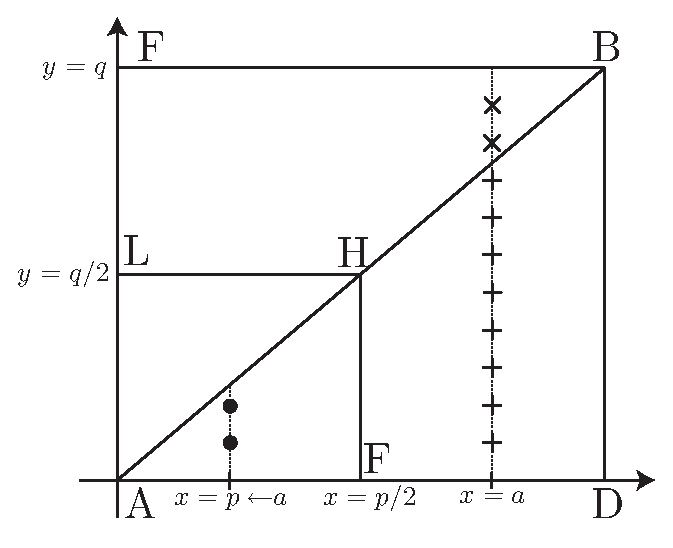
\includegraphics [scale = 0.7]{images/demo-geom-reciprocite.eps}
    \end{center}
    \caption{Geometric proof of the quadratic reciprocity law}
              \label{fig-demo-geom-reciprocite}
\end{figure}
\end{exo}
 
 
\begin{exo}[Fermat's theorem on a finite field]
\label{exo-thm-fermat-finite-body}
 
\index{Fermat's equation} \index{Fermat@\nompropreindex{Fermat}} This exercise uses the notations and results of the exercise \oldref{exo-eqn-grpe-abelien-finite}. Let $ q = p^r $ where $ p $ is a prime number. We want to show that if $ k $ is an integer such that $ q \geq k^4 + 4 $, then Fermat's equation on $ \FF_q $
\begin{equation}
\label{eq-thm-fermat-finite-body}
x^k + y^k = z^k \quad \quad \quad x, \, y, \, z \in \FF_q^*
\end{equation}
has a solution. To do this, we will use the Fourier transform on the group $ (\FF_q, \, +) $. \begin{enumerate}
\item \index{Subgroup} Let $ k | q-1 $. Show that there exists a unique subgroup $ H_k $ of index $ k $ in $ \FF_q^* $ and that
\begin{equation*}
H_k = \enscond{x^k}{x \in \FF_q^*}.
\end{equation*}
 
\item \index{Group!quotient} We denote by $ \chi_0, \ldots, \, \chi_{k-1} $ the multiplicative characters of the quotient group $ \FF_q^* / H_k $. They are canonically extended into multiplicative characters of $ \FF_q^* $ by composing by the canonical projection. Show then that for any additive character $ \psi $ we have
\begin{equation*}
\wh{f_{H_k}} (\psi) = \frac{1}{k} \sum_{i = 0}^{k-1}{G (\chi_i, \, \psi)}.
\end{equation*}
Using the proposition \ref{prop-calcul-sums-gauss}, show then that $ \Phi (H_k) <\sqrt{q} $, where $ \Phi $ is defined by the equation \eqref{eq-defn-phi-ensemble}.
\item Let $ A_1, \, A_2 \subset G $. We denote by $ N $ and $ N'$ respectively the number of solutions of the equations
\begin{align}
\label{eq-thm-fermat_intermediaire}
x + y & = z^k, \quad \quad & \text{with} \quad x \in A_1, \; y \in A_2, \; z \in \FF_q^*, \\
x + y & = u, \quad \quad & \text{with} \quad x \in A_1, \; y \in A_2, \; u \in H_k.
\end{align}
Show that $ N = k N'$, then show that
\begin{equation}
\label{eqn-fermat-majoration}
\left| N - \frac{| A_1 | | A_2 | (q-1)}{q} \right| <k \sqrt{| A_1 | | A_2 | q}.
\end{equation}
We can start by proving a similar inequality for $ N'$ using the result of the exercise \oldref{exo-eqn-grpe-abelien-finite}, question 2.
\item If we denote by $ l_i \eqdef \frac{q-1}{| A_i |} $, then show that if $ q \geq k^2 l_1 l_2 + 4 $ the equation \eqref{eq-thm-fermat_intermediaire} admits a solution. In the case where $ k $ does not divide $ q-1 $, show that
\begin{equation*}
\enscond{x^k}{x \in \FF_q^*} = \enscond{x^d}{x \in \FF_q^*},
\end{equation*}
where $ d \eqdef \PGCD (q-1, \, k) $. Deduce that the result is valid for any $ k $ satisfying $ q \geq k^2 l_1 l_2 + 4 $.
\item Using the sets $ A_1 = A_2 = H_k $, show that if $ q \geq k^4 + 4 $, then the equation \eqref{eq-thm-fermat-finite-body} admits at least one solution .
\end{enumerate}
\end{exo}
 
 
\begin{exo}[Walsh transform and statistical study]
\label{exo-transforme-walsh-statistic}
 
This exercise is taken from an article by \nompropre{Rockmore} and \nompropre{Malsen}{\upshape \cite{rockmore-generalized}}, which presents a technique known as the analysis of \textit{Yates}, from the name of the statistician who invented this method. Consider the following situation: a farmer wants to know the influence of three parameters on his wheat production. These parameters are the lighting (represented by the variable $ a $), the amount of herbicide (variable $ b $), and the amount of fertilizer (variable $ c $). Each of these variables can take two values: high quantity (noted $ + $) and low quantity (noted $ - $). An experimental report is given in the form of the following table grouping the values for the average size of wheat (in centimeters) under the different conditions:
\begin{equation*}
\begin{array}{c | c | c || c} a & b & c & \alpha_{abc} \\\hline + & + & + & 69 \\- & + & + & 81 \\+ & - & + & 63 \\- & - & + & 77 \\+ & + & - & 61 \\- & + & - & 92 \\+ & - & - & 54 \\- & - & - & 89 \end{array}
\end{equation*}
We can therefore represent these results in the form of a function
\begin{equation*}
f: \func{(\ZZ/2 \ZZ)^3 \simeq \{-, +\}^3}{\RR}{(a, \, b, \, c)}{\alpha_{abc} }.
\end{equation*}
In order to analyze these results, we define the 0-order interaction, denoted $ \mu $, which is simply the mean:
\begin{equation*}
\mu \eqdef \frac{1}{8} \sum_{(a, \, b, \, c) \in \{+, -\}^3}{\alpha_{abc}}.
\end{equation*}
We then define the interactions of order 1, denoted $ \mu_a $, $ \mu_b $ and $ \mu_c $, as corresponding to the effect of a single parameter, the other two being assumed to be constant. For example we have
\begin{equation*}
\mu_{a} \eqdef \frac{1}{4} \sum_{(b, \, c) \in \{+, -\}^2}{\alpha_{+ bc}} - \frac{1 }{4} \sum_{(b, \, c) \in \{+, -\}^2}{\alpha_{- bc}}.
\end{equation*}
In the same vein, define the 3 interactions of order 2, denoted by $ \mu_{ab} $, $ \mu_{bc} $ and $ \mu_{ac} $, as well as the interaction of order 3, denoted by $ \mu_{abc} $. How can we calculate all these interactions using the Walsh transform? Deduce a fast calculation algorithm. Do the math for the farmer.
\end{exo}
 
 
\begin{exo}[Haar wavelet]
\label{exo-wavelet-haar}
 
\index{Wavelet!of Haar} \index{Haar@\nompropreindex{Haar}} \index{Base!orthonormal} \index{Base!of Haar} \index{Base!of Hilbert} We denote $ \psi_0 $ the function indicator of $ [0, \, 1] $ and $ \psi $ the function which is worth $ 1 $ on $ [0, \, \frac{1}{2}[$, $ -1 $ on $ [\frac{1}{2}, \, 1] $, and $ 0 $ everywhere else. We then define a series of functions $ \psi_n $ by
\begin{equation*}
\forall j \geq 1, \; \forall k \in \{0, \ldots, \, 2^{j-1} -1\}, \quad \psi_n (x) \eqdef \psi_{j, k} (x) \eqdef 2^{\frac{j}{2}} \psi \left(2^jx - k \right),
\end{equation*}
where $ n = 2^{j-1} + k $. We denote, for $ j \geq 0 $, $ F_j $ the space of functions of $ [0, \, 1] $ in $ \RR $ constants on each of the intervals $ I_k \eqdef [k 2^{- j }, \, (k + 1) 2^{- j}[$, for $ k \in \{0, \ldots, \, 2^j-1\} $ (we include the point $ 1 $ in the last interval). \begin{enumerate}
\item Show that $ \left\{\psi_n \right\}_{n = 0}^{2^j-1} $ forms an orthonormal basis of $ F_j $ for the usual scalar product of $ L^2 ([ 0, \, 1]) $.
\item Let $ f $ be a continuous function of $ [0, \, 1] $ in $ \RR $. For $ J \geq 0 $, we denote by $ f_J $ the projection of $ f $ on $ F_J $:
\begin{equation*}
f_J \eqdef \sum_{j = 0}^J{\sum_{k = 0}^{2^{j-1} -1}{\dotp{f}{\psi_{j, k}} \psi_{j, k}}}.
\end{equation*}
Show that $ f_J $ converges uniformly on $ [0, \, 1] $ to $ f $ when $ J \rightarrow + \infty $. We then define, for $ n \geq 0 $, the function
\begin{equation*}
\wt{f}_n \eqdef \sum_{m = 0}^{n}{\dotp{f}{\psi_m} \psi_m}.
\end{equation*}
Show that $ \wt{f}_n $ converges uniformly to $ f $ when $ n \rightarrow \infty $. Then show that $ \{\psi_n\}_{n \in \NN} $ forms a Hilbert basis of $ L^2 ([0, \, 1]) $. The figure \figref{fig-decomposition-base-haar} represents the decomposition of a function $ f $ on the first vectors of the base of $ \psi_n $, which we call the Haar base. \begin{figure}[ht]
    \begin{center}
    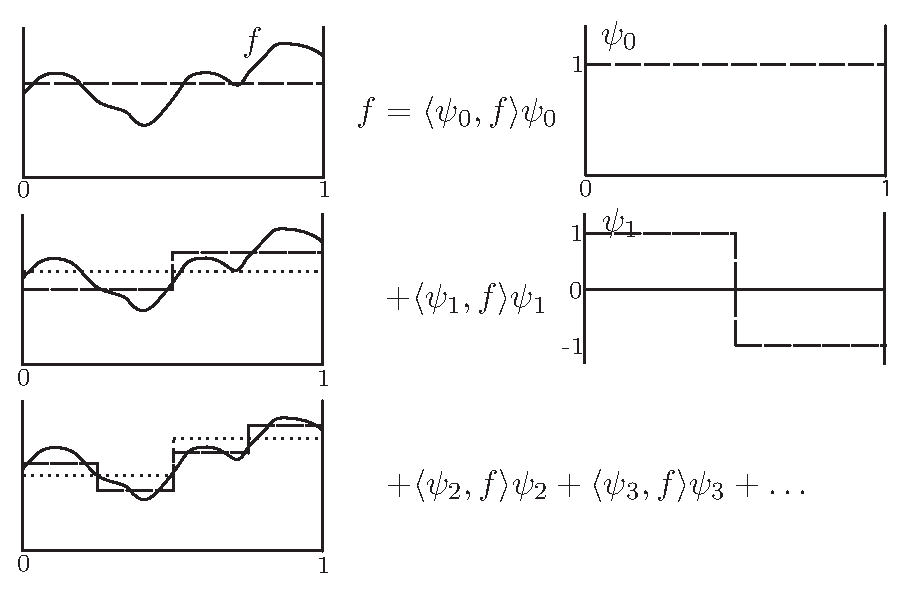
\includegraphics [scale = 0.8]{images/decomposition-base-haar.eps}
    \end{center}
    \caption{Decomposition based on Haar}
              \label{fig-decomposition-base-haar}
\end{figure}
 
\item We introduce, for $ j \geq 0 $, the functions \guill{stepped} $ \varphi_{j, k} (x) \eqdef 2^{\frac{j}{2}} \psi_0 \left(2^jx - k \right) $. Show that $ \varphi_{j, k} $, for $ k \in \{0, \ldots, \, 2^j-1\} $, forms an orthonormal basis of $ F_j $. We define $ G_{j-1} $ the vector space such that $ F_j = F_{j-1} \oplus G_{j-1} $ (space of \guill{details}). Show that $ \{\psi_{j, k}\}_{k = 0}^{2^{j-1} -1} $ is an orthonormal basis of $ G_{j-1} $. Then express the function $ \psi_{j, k} $ as a linear combination of $ \varphi_{j + 1, s} $, $ s \in \{0, \ldots, \, 2^j-1 $.
\item Let $ f \in F_j $. We denote by $ x^{(0)} \in \RR^{2^j} $ the vector of scalar products $ x^{(0)}[k] = \dotp{f}{\varphi_{j, k }} $. How do you calculate them from $ f $? For $ i \in \{1, \ldots, \, j\} $, we define vectors $ x^{(i)} $ and $ d^{(i)} $ of size $ 2^{ji} $ , by the relations, for $ k \in \{0, \ldots, \, 2^{ji} -1\} $,
\begin{align*}
x^{(i)}[k] & \eqdef \frac{x^{(i-1)}[2k + 1] + x^{(i-1)}[2k]}{\sqrt{2} } \\
d^{(i)}[k] & \eqdef \frac{x^{(i-1)}[2k + 1] - x^{(i-1)}[2k]}{\sqrt{2} }.
\end{align*}
\index{Rotation} \index{Signal} Intuitively, $ x^{(i)} $ represents the trend in the signal $ x^{(i-1)} $, and $ d^{(i)} $ represents the details. The figure \figref{fig-decomposition-wavelet-haar} symbolizes the succession of calculations to be performed to obtain the vectors $ d^{(i)} $ as well as the last coefficient $ x^{(j)}[0] $ . Show that the operator $ x^{(i)} \mapsto (x^{(i + 1)}, \, d^{(i + 1)}) $ can be seen as an isometry (more precisely a rotation ) of $ \RR^{ji} $. Show that the $ x^{(i)} $ all have the same average, and therefore that $ x^{(j)}[0] $ represents the average of the original $ x^{(0)} $ signal . 

\begin{figure}[ht]
    \begin{center}
    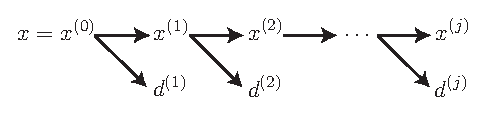
\includegraphics[scale=1.0]{images/decomposition-ondelette-haar.eps}
    \end{center}
    \caption{Cascade calculation of the decomposition coefficients}
              \label{fig-decomposition-wavelet-haar}
\end{figure}
 
\item Show that we have, for $ i \in \{1, \ldots, \, j\} $ and for $ k \in \{0, \ldots, \, 2^{ji} -1\} $,
\begin{equation*}
d^{(i)}[k] = \dotp{f}{\psi_{j-i + 1, k}} \quad \quad \text{and} \quad \quad x^{(j)}[ 0] = \dotp{f}{\psi_0}.
\end{equation*}
Thanks to this algorithm, what is the number of operations necessary to decompose a function of $ F_j $ on the basis of $ \psi_n $?
\item \index{Complexity} We assume that $ n = 2^j $. Show that the operator $ \Gamma $ which to $ x \in \RR^{n} $ associates the vector $ (d^{(1)}, \, x^{(2)}, \ldots, \, d^{(j)}, \, x^{(j)}) $ is an isometry of $ \RR^{n} $ for the canonical dot product (we put the vectors $ d^{( i)}, \, x^{(i)}, \ldots $). Deduce that the application of this operator corresponds to the decomposition of $ x $ in an orthonormal basis of $ \RR^{n} $ that we will specify. Compare this database to the Walsh database described in paragraph~\ref{sect2-presentation-transforme-walsh}. Compare in terms of complexity the algorithm of decomposition in the base of Haar and that of decomposition in the base of Walsh (FWT algorithm, paragraph~\ref{sect2-fwt}).
\end{enumerate} Figure \figref{fig-transforme-haar} shows two examples of transforms $ y = \Gamma x $. We can see that since the signals are regular, only the coefficients corresponding to the coarse scales (that is to say for $ j $ small, the indices on the right of the transform) are large. \begin{figure}[ht]
    \begin{center}
    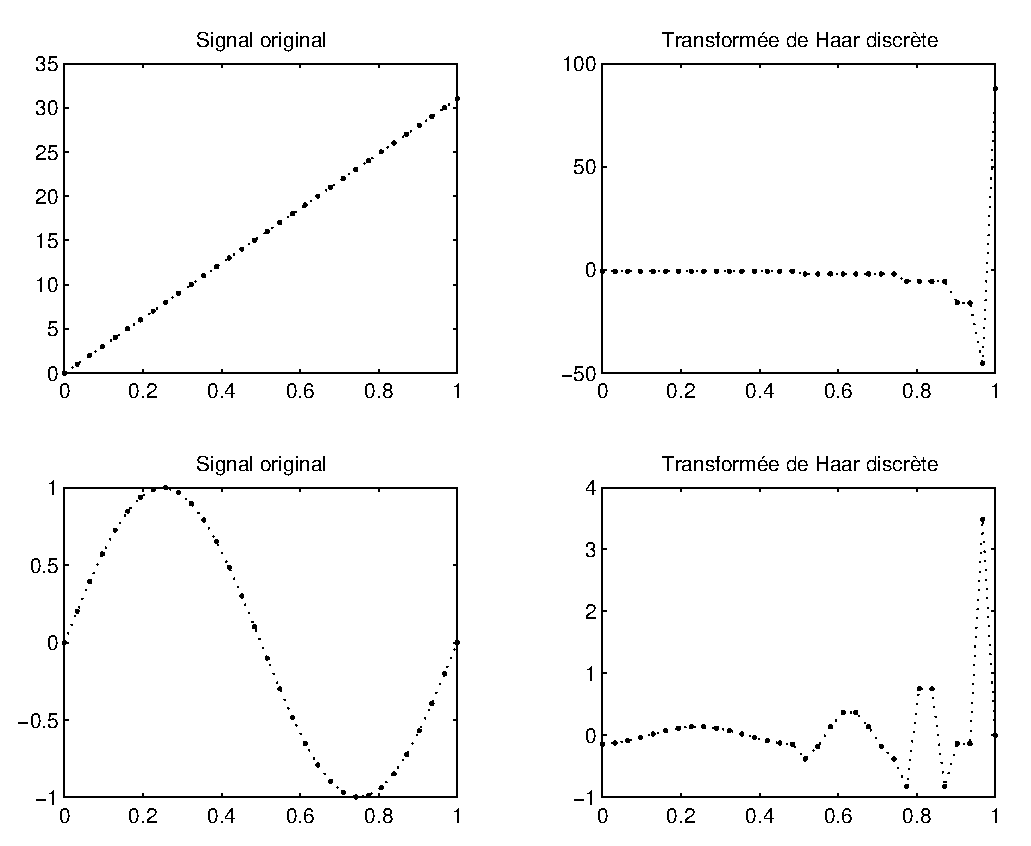
\includegraphics [scale = 0.7]{images/transformee-haar.eps}
    \end{center}
    \caption{Examples of discrete Haar transforms}
              \label{fig-transforme-haar}
\end{figure}
The Haar base is the simplest example of a wavelet base. The fast wavelet transformation algorithm was introduced by \nompropre{Mallat},{\upshape \cite{mallat}}. The differences between the Walsh and Haar bases illustrate the transition from the Fourier transform (here on $ (\FF_2)^k $) to the wavelet transform. The exercise \oldref{exo-wavelets-finite-fields} presents the construction of wavelets on finite fields.
\end{exo}
 
 
\begin{exo}[Image compression]
\label{exo-compression-walsh}
\index{Compression} The goal of this exercise is to properly order Walsh functions to successfully compress 1D and 2D signals. \begin{enumerate}
\item \index{2D Walsh transform} Generalize the discrete Walsh transform to the two-dimensional case. We will use the functions
\begin{equation*}
\chi_{i, \, j} (s, \, t) = \chi_i (s) \chi_j (t).
\end{equation*}
Write a fast computation algorithm for the 2D Walsh transform.
\item Show that we can classify the discrete Walsh functions (defined by the equation \eqref{eq-denf-base-walsh}) in increasing order of the number of sign changes. The figure \figref{fig-functions-walsh} shows the Walsh matrices obtained by classifying the functions in the usual order and in the order of the number of sign changes. \begin{figure}[ht]
    \begin{center}
    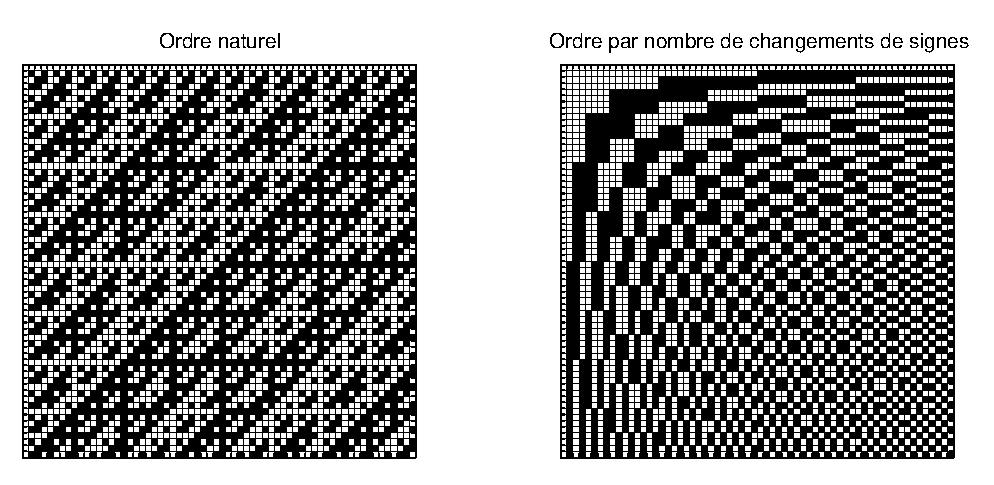
\includegraphics [scale = 0.7]{images/fonctions-walsh.eps}
    \end{center}
    \caption{Two ways to classify Walsh functions}
              \label{fig-functions-walsh}
\end{figure}
 
\item \index{Signal} Intuitively, such a classification makes it possible to order the Walsh spectrum from tendencies (low frequencies) to details (high frequencies). Calculate for some functions the spectra obtained with the two classifications, and verify this interpretation. The figure \figref{fig-spectrum-walsh-1d} shows the spectra of the function represented at the top left of the figure \figref{fig-compression-walsh-1d}. 

\begin{figure}[ht]
    \begin{center}
    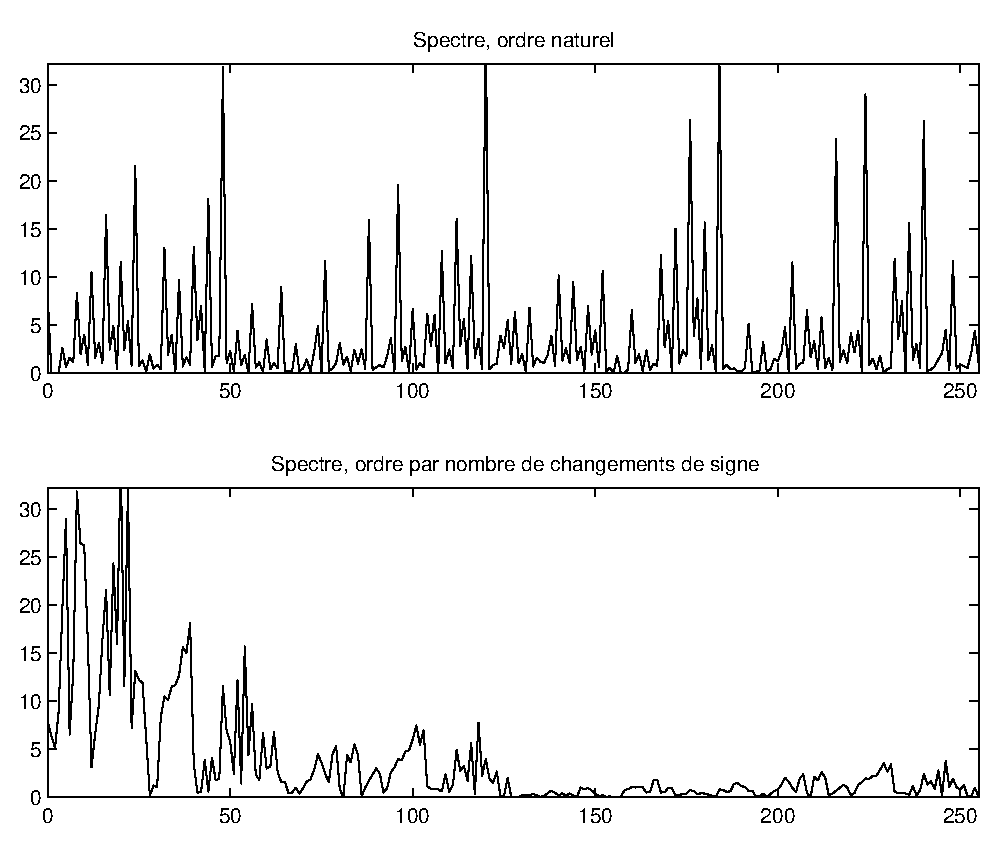
\includegraphics[scale = 0.5]{images/spectre-walsh-1d.eps}
    \end{center}
    \caption{Walsh spectrum of a 1D signal}
              \label{fig-spectrum-walsh-1d}
\end{figure}
 
\item We have therefore classified the Walsh functions according to an order $ \chi_{i_0}, \ldots, \, \chi_{i_N} $. We consider a signal $ f \in \CC^N $. For $ 0 \leq n <N $, we construct the function
\begin{equation*}
f_n \eqdef \sum_{k = 0}^{n}{\dotp{f}{\chi_{i_k}} \chi_{i_k}}.
\end{equation*}
Explain why this process allows to compress the signal $ f $. Figure \figref{fig-compression-walsh-1d} shows the progressive compression of a signal. The percentage of Walsh coefficients which have been retained is indicated each time. After studying the discrete Fourier transform in chapter \oldref{chap-tfd}, we can perform the same process, but with the Fourier spectrum. What are the advantages and disadvantages of each method (calculation time, quality of reconstruction, etc.)? \begin{figure}[ht]
    \begin{center}
    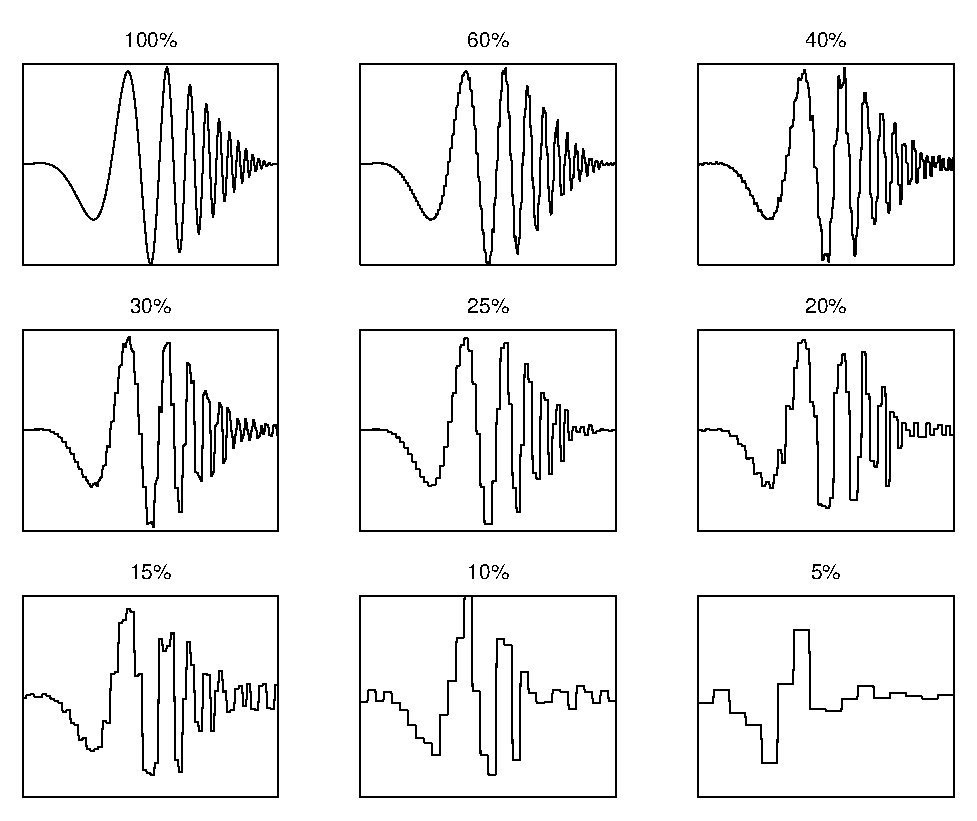
\includegraphics [scale = 0.6]{images/compression-walsh-1d.eps}
% \includegraphics [scale = 0.6]{images/compression-walsh-1d-2.eps}
    \end{center}
    \caption{Compression of a 1D signal}
              \label{fig-compression-walsh-1d}
\end{figure}
 
\item What classification (s) can we adopt for the functions of Walsh 2D? The figure \figref{fig-functions-walsh-2d} proposes such a classification (from left to right and top to bottom). \begin{figure}[ht]
    \begin{center}
    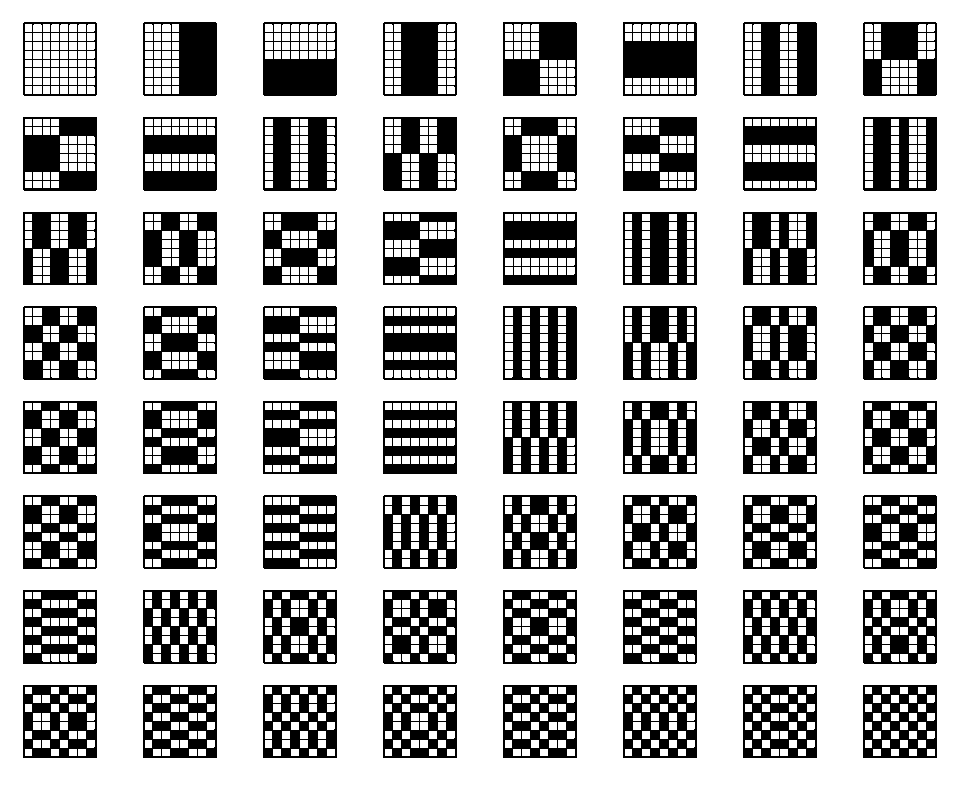
\includegraphics [scale = 0.6]{images/fonctions-walsh-2d.eps}
    \end{center}
    \caption{Classification of 2D Walsh functions}
              \label{fig-functions-walsh-2d}
\end{figure}
Apply this classification to compress 2D images. Write a \Matlab{} program to perform this compression. The figure \figref{fig-compression-walsh-2d} shows the progressive compression of an image representing the letter A. \begin{figure}[ht]
    \begin{center}
    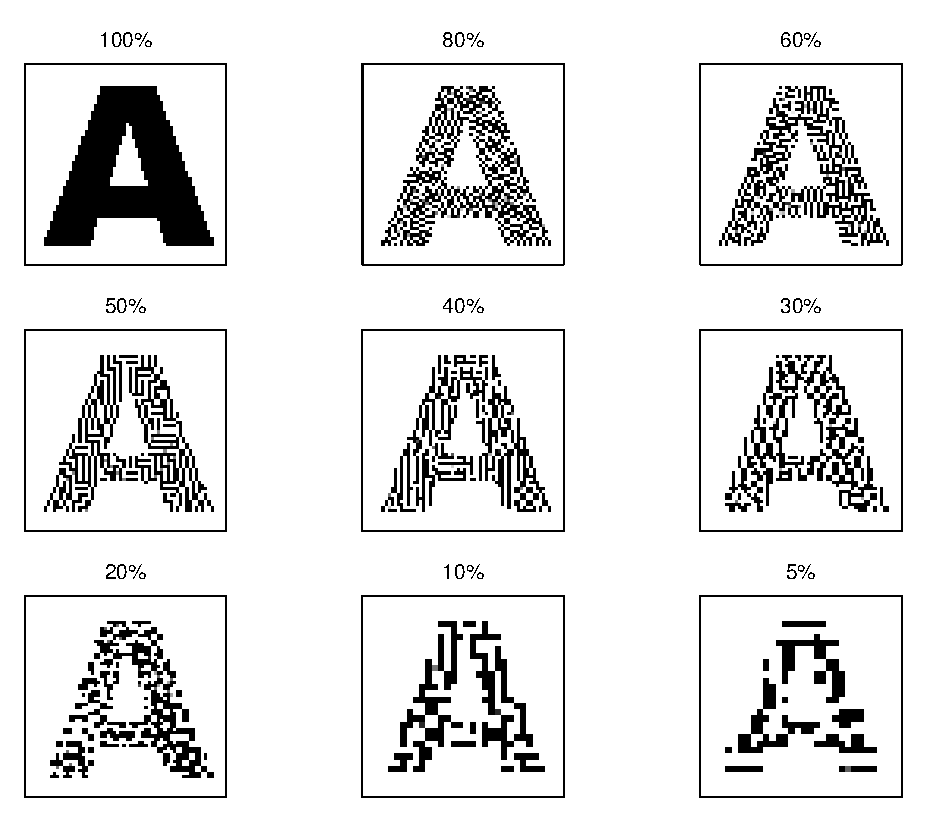
\includegraphics [scale = 0.6]{images/compression-walsh-2d.eps}
% \includegraphics [scale = 0.6]{images/compression-walsh-2d-2.eps}
    \end{center}
    \caption{Compress a 2D image}
              \label{fig-compression-walsh-2d}
\end{figure}
\end{enumerate}
\end{exo}
 
 
\begin{exo}[Hadamard matrices]
\label{exo-matrices-hadamard}
\index{Matrix!of Hadamard} \index{Hadamard@\nompropreindex{Hadamard}} \index{Determinant!maximal} This exercise makes the connection between the Walsh matrices considered in paragraph~\ref{sect2-presentation-transforme-walsh} and the quadratic residuals introduced at the beginning of this chapter. A matrix $ H_n $, of size $ n \times n $, whose inputs are $ + 1 $ or $ -1 $, is called a Hadamard matrix if it satisfies
\begin{equation*}
H_n \transp{H_n} = n \Id_n,
\end{equation*}
where we denote by $ \transp{H_n} $ the transposed matrix of $ H_n $. \begin{enumerate}
\item Explain why the matrix $ W_n $, defined in the proposition \ref{prop-pte-matrix-hadamard}, for $ n = 2^k $, is a Hadamard matrix.
\item Show that if there exists a Hadamard matrix $ H_n $ of size $ n \times n $, then $ n $ is worth $ 1 $, or $ 2 $, or is a multiple of $ 4 $. We can start by showing that we can assume that $ H_n $ is normalized, that is to say with $ 1 $ on the first row and the first column. Then we will show that if $ n \geq 3 $, we can assume that the first three lines of $ H_n $ are written in the form
\begin{equation*}
\begin{array}{cccc} \underbrace{\begin{matrix} 1 & \ldots & 1 \\1 & \ldots & 1 \\1 & \ldots & 1 \end{matrix}} & \underbrace{\begin{matrix} 1 & \ldots & 1 \\1 & \ldots & 1 \\-1 & \ldots & -1 \end{matrix}} & \underbrace{\begin{matrix} 1 & \ldots & 1 \\-1 & \ldots & -1 \\1 & \ldots & 1 \end{matrix}} & \underbrace{\begin{matrix} 1 & \ldots & 1 \\-1 & \ldots & -1 \\- 1 & \ldots & -1 \end{matrix}} \\i & j & k & l \end{array}
\end{equation*}
where the integers $ i $, $ j $, $ k $, and $ l $ denote the lengths of each portion (they can optionally be zero). Finally, we will show that we actually have $ i = j = k = l $.
\item \index{Paley@\nompropreindex{Paley}} \index{Matrix!of Paley} \index{Quadratic residue} The inverse problem, namely the construction of a matrix $ H_n $ for a $ n $ multiple of $ 4 $ given, is very complex. In fact, it is speculated that it is still possible to do so, although it has not yet been proven. Assume that $ n = p + 1 $, where $ p $ is an odd prime number. We also suppose that $ n $ is a multiple of $ 4 $, and we will show that we can then construct a matrix $ H_n $. We will use the quadratic residue character modulo $ p $, denoted by $ \eta $, which is defined in the equation \eqref{eq-defn-cartactere-eta}. We define a matrix $ Q $ of size $ p \times p $ by
\begin{equation*}
Q \eqdef \left\{\eta (ji) \right\}_{0 \leq i, \, j \leq p-1}.
\end{equation*}
Show that $ Q $ is anti-symmetric, and that we have $ Q \transp{Q} = p \Id_p - J $, where $ J $ is the matrix whose all inputs are worth $ 1 $. Also show that we have $ QJ = JQ = 0 $. Such a matrix is called \textit{Paley matrix}.
\item We now define the matrix $ H_n $ of size $ n \times n $ by
\begin{equation*}
H_n \eqdef \begin{pmatrix} 1 & v \\\transp{v} & Q- \Id_p \end{pmatrix},
\end{equation*}
where we noted $ v = (1, \ldots, \, 1) \in \RR^p $. Show that $ H_n $ is a Hadamard matrix. Here is an example for $ p = $ 7:
\begin{equation*}
H_8 \eqdef \begin{pmatrix} 1 & 1 & 1 & 1 & 1 & 1 & 1 & 1 \\1 & -1 & 1 & 1 & -1 & 1 & -1 & -1 \\1 & -1 & -1 & 1 & 1 & -1 & 1 & -1 \\1 & -1 & -1 & -1 & 1 & 1 & -1 & 1 \\1 & 1 & -1 & -1 & -1 & 1 & 1 & -1 \\1 & -1 & 1 & -1 & -1 & -1 & 1 & 1 \\1 & 1 & -1 & 1 & -1 & -1 & -1 & 1 \\1 & 1 & 1 & -1 & 1 & -1 & -1 & -1 \end{pmatrix}.
\end{equation*}
 
\item Let $ A $ be a matrix of size $ n \times n $ such that its inputs $ a_{ij} $ verify
\begin{equation*}
\forall (i, \, j) \in \{1, \ldots, \, n\}^2, \quad | a_{ij} | \leq 1.
\end{equation*}
Show the Hadamard inequality:
\begin{equation}
\label{eq-borne-hadamard}
| \det (A) | \leq n^{\frac{n}{2}}.
\end{equation}
Show that if there is a Hadamard matrix, then the latter reaches this bound.
\end{enumerate} The geometric interpretation of the bound \eqref{eq-borne-hadamard} is very simple. It is a matter of considering a system of $ n $ vectors (the columns of the matrix) inside the cube $ | x_i | \leq 1 $, (where we denote by $ \{x_i\}_{i = 1}^n $ a coordinate system), enclosing a rectangular parallelepiped of maximum volume. In the case of Hadamard matrices, these vectors are large diagonals of the cube, and therefore have maximum lengths. In addition, they are orthogonal, so as to produce the maximum volume. In dimensions where Hadamard matrices do not exist, it is not possible to produce orthogonal diagonals, even if one thinks that the vectors which minimize \eqref{eq-borne-hadamard} are close to the large diagonals . This remains an open problem. \\The exercise \oldref{exo-codes-hadamard} presents an application of Hadamard matrices for the construction of bi-orthogonal corrective codes.
\end{exo}
 
 
\begin{exo}[Matrix tensor product]
\label{exo-tensor-product}
\index{Tensor product} Let $ A $ be a square matrix of size $ s $ and $ B $ a square matrix of size $ t $. We define the tensor product $ A \otimes B $ as the matrix of size $ s \times t $
\begin{equation*}
A \otimes B \eqdef \begin{pmatrix} a_{11} B & \cdots & a_{1s} B \\\vdots & & \vdots \\a_{s1} B & \cdots & a_{ss} B \end{pmatrix}.
\end{equation*}
\begin{enumerate}
\item We assume that $ A $ matches $ AA^* = s \Id_s $. Show that $ A^{\otimes n} = A \otimes \cdots \otimes A $ ($ n $ products) satisfies $ A^{\otimes n} (A^{\otimes n})^* = s^n \Id_{s^n} $.
\item What is the connection with the Walsh transform?
\item Taking inspiration from the fast FWT algorithm, write a fast algorithm that computes the transform $ y = A^{\otimes n} x $. How is the inverse transform calculated?
\item We take as base matrix
\begin{equation*}
A_\alpha \eqdef \sqrt{2} \begin{pmatrix} \cos (\alpha) & \sin (\alpha) \\\sin (\alpha) & - \cos (\alpha) \end{pmatrix}.
\end{equation*}
How can the transform $ x \mapsto A_\alpha^{\otimes n} x $ be seen as an intermediate Walsh transform?
\end{enumerate} The figure \figref{fig-transfo-walsh-interm} shows the transforms of a \guill{triangle} function for values of $ \alpha $ in $ [0, \pi / 2] $. The ordinary Walsh transform corresponds to the \ordin{6}{th} curve. For $ \alpha = \pi / 2 $, we find the original symmetrized signal. \begin{figure}[ht]
    \begin{center}
    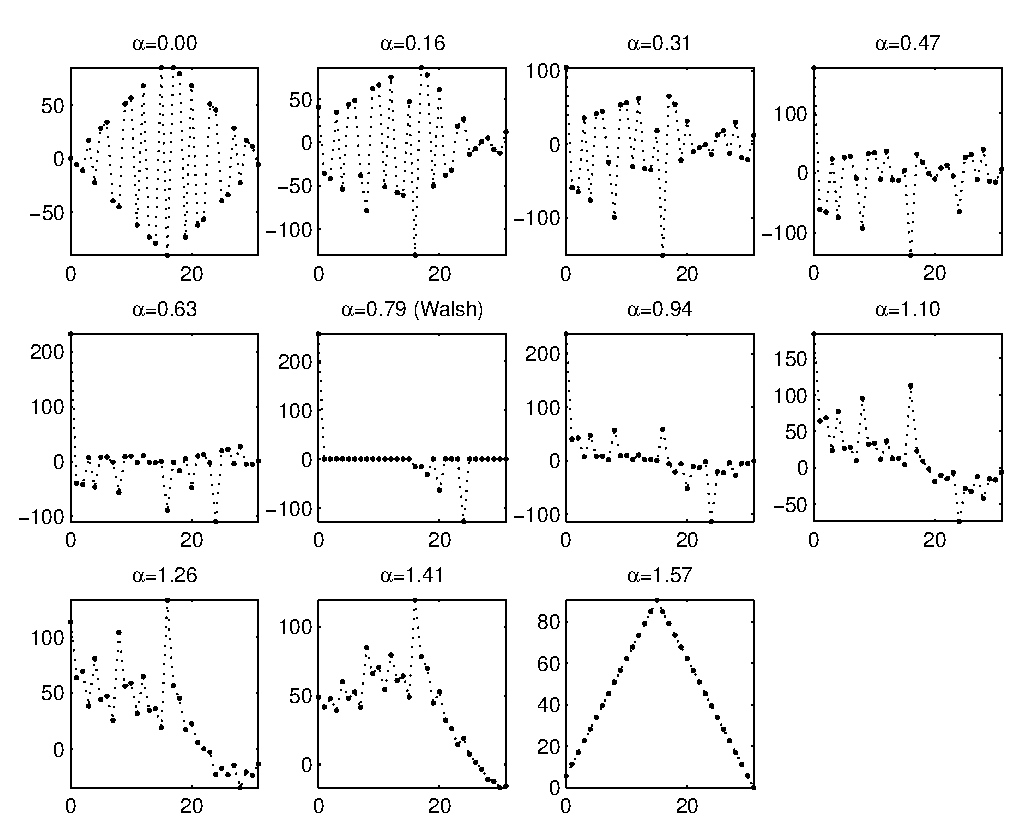
\includegraphics [scale = 0.7]{images/transfo-walsh-interm.eps}
% \includegraphics [scale = 0.7]{images/transfo-walsh-interm-2.eps} BUG?
    \end{center}
    \caption{Intermediate Walsh transform}
              \label{fig-transfo-walsh-interm}
\end{figure}
We can look at the exercise \oldref{exo-grpe-quaternionique}, which uses the theory of linear representations to build a matrix $ A $ of size $ 8 $.
\end{exo}
 
 
\begin{exo}[Generalization of the identity of MacWilliams]
\label{exo-generalization-mac-williams}
 
\index{MacWilliams@\nompropreindex{MacWilliams}} \index{Identity!of MacWilliams} In this exercise, we propose to extend the identity of MacWilliams to the case of the vector space $ E = \FF_q^k $. \begin{enumerate}
\item We define the following bilinear form on $ E \times E $, with value in $ \FF_q $:
\begin{equation*}
\forall (a, \, x) \in E^2, \quad \dotp{a}{x} \eqdef \sum_{i = 0}^{p-1}{a_i x_i}.
\end{equation*}
Explain how it represents the bilinear form of the duality (bracket of the duality) between the space $ E $ and its dual $ E^* $ (correctly identified as $ E $).
\item We denote by $ \chi_1 $ the canonical additive character of $ \FF_q $, as defined by the equation \eqref{defn-character-additive-canonical}. Let $ a = \{a_0, \ldots, \, a_{k-1}\} \in (\ZZ/q \ZZ)^k $. We define
\begin{equation*}
\chi_a: \func{E}{\CC^*}{x}{\chi_1 (\dotp{a}{x})}.
\end{equation*}
Explain why the applications $ \chi_a $ allow to define an isomorphism between $ E $ and its dual as an additive group, $ \wh{E} $.
\item \index{Subgroup} \index{Orthogonal!of a vector space} \index{Orthogonal!of a subgroup} Let $ H $ be a subgroup of $ E $. Show that it is also a vector subspace. Deduce from the previous question that we can identify the orthogonal of $ H $ for the group structure, noted $ H^{\sharp} $, and that for the vector space structure, noted $ H^{\bot} $.
\item Demonstrate the identity of MacWilliams within the $ E $ space:
\begin{equation*}
A_{H^{\bot}} (X, \, Y) = \frac{1}{| H |} A_{H} (X + (q-1) Y, \, XY).
\end{equation*}
\end{enumerate}
\end{exo}
 
 
\begin{exo}[Poisson formula and distributions]
\label{exo-formula-fish-distrib}
\index{Distribution} \index{Dirac comb} \label{notation-41} This exercise requires some knowledge of distribution theory, in particular the definition of the Fourier transform of a distribution. Here we take as convention the transform defined in the equation \eqref{eq-transforme-fourier-R}, which differs by a factor of $ 2 \pi $ from that used in \eqref{eq-defn-trans-fourier-special-fish}. We denote by $ \Pi_s $ the Dirac comb of steps $ s $, that is to say
\begin{equation}
\label{eq-trans-fourier-comb-dirac}
\Pi_s \eqdef \sum_{k \in \ZZ}{\delta_{ks}},
\end{equation}
\index{Support!compact} where $ \delta_t $ is the distribution defined by $ \dotp{\delta_t}{\varphi} \eqdef \varphi (t) $ for $ \varphi \in \Cc^\infty_0 (\RR ) $ (functions of class $ \Cc^\infty $ with compact support). Show that the Poisson formula \eqref{eq-formula-fish-continue} implies the following equality:
\begin{equation*}
\wh{\Pi_s} = \frac{2 \pi}{s} \Pi_{\frac{2 \pi}{s}}.
\end{equation*}
\end{exo}
 
 
\begin{exo}[Shannon sampling]
\label{exo-sample-shannon}
 
\index{Shannon@\nompropreindex{Shannon}} \index{Sampling!theorem} \index{Sampling} Let $ T> 0 $. We notice
\begin{equation*}
I_T \eqdef \left[- \frac{\pi}{T}, \, \frac{\pi}{T} \right] \quad \text{et} \quad E_T \eqdef \enscond{f \in L^2 (\RR)}{\Supp (\wh{f}) \subset I_T}.
\end{equation*}
Let $ f \in E_T $. We want to prove Shannon's sampling theorem, which says that $ f $ can be reconstructed (interpolated) from the samples $ f(n T) $, for $ n \in \ZZ $. More precisely, if we note
\begin{equation}
\label{eqn-formula-reconstruction-shannon}
\sinc_T (t) \eqdef \frac{\sin \left(\ofrac{\pi t}{T} \right)}{\ofrac{\pi t}{T}},
\end{equation}
so we want to show that
\begin{equation*}
f(t) \eqdef \sum_{n \in \ZZ}{f(n T) \sinc_T (tn T)}.
\end{equation*}
\begin{enumerate}
\item Show that $ f $ is of class $ \Cc^\infty $.
\item We denote by $ f_d $ the distribution which corresponds to the sampling of $ f $:
\begin{equation*}
f_d \eqdef \sum_{n \in \ZZ}{f(n T) \delta_{n T}}.
\end{equation*}
Using the equality \eqref{eq-trans-fourier-comb-dirac}, show that we have
\begin{equation*}
| \omega | \leq \frac{\pi}{T} \Longrightarrow \wh{f_d} (\omega) = \frac{1}{T} \wh{f} (\omega).
\end{equation*}
 
\item Calculate the inverse Fourier transform of the indicator function of the interval $ I_T $. Deduce the sampling theorem.
\item \index{Hilbert basis} \index{Orthogonal!projection} Show that the family $ \{t \mapsto \sinc_T (t n T)\}_{n \in \ZZ} $ forms an orthogonal base (base de Hilbert) of the space $ E_T $. How is the projection of a function $ f \in L^2 (\RR) $ calculated on this space?
\end{enumerate}
\end{exo}
